%% 
%% Author: Alvaro Santamaria Herrero
%%
%% LaTeX template based on:
%% V1.0
%% by Gabriel Garcia, gabrcg@gmail.com
%% This is a template for Udacity projects using IEEEtran.cls
%%

%% Be Udacious!

\documentclass[10pt,journal,compsoc, onecolumn]{IEEEtran}

\usepackage[pdftex]{graphicx}    

\usepackage[utf8]{inputenc}
\usepackage{hyperref}
\usepackage{multicol,caption}
\usepackage{datetime}
\usepackage{listings}
\usepackage{verbatim}
%\usepackage{cite}
\usepackage[style=numeric, citestyle=numeric]{biblatex}
\usepackage{dirtytalk}

\bibliography{bib}
\newdateformat{monthyeardate}{\monthname[\THEMONTH], \THEYEAR}
\hyphenation{op-tical net-works semi-conduc-tor}
%\setlength{\arrayrulewidth}{1mm}
%\setlength{\tabcolsep}{18pt}
\renewcommand{\arraystretch}{1.5}
\setcounter{tocdepth}{2}




\begin{document}


\title{Multi-Class Text Classification with \\Convolutional Neural Nets}
\author{Álvaro Santamaría Herrero\\\vspace*{10pt} \normalsize  Udacity Machine Learning Engineer Nanodegree\\ Capstone Project Report\\\monthyeardate\today}

\markboth{Natural Language Processing, Convolutional Neural Nets, Machine Learning, Nanodegree, Udacity}%
{}

\IEEEtitleabstractindextext{%

\begin{abstract}
We built and trained a convolutional neural net (CNN) to perform multi-class text classification on the well-known 20-class \textit{20 Newsgroups} corpus. On top of evaluating the performance of the model, we tried to quantify how much of it can be attributed to the ability to extract information that is \textit{positionally encoded} in text sequences. In order to help with that, and together with \textit{accuracy}, we proposed \textit{information gain} as a companion score to evaluate model performance. As a benchmark we compared the model with two carefully trimmed-down versions of itself that, by design, cannot extract positional information. We also compared our model to a baseline Multinomial Naïve Bayes classifier. Our proposed model proved to have modest although statistically significant gain in performance that can be attributed to extraction of positional information (0.050 bits). It also improved 3.8\% in accuracy and gained 0.105 bits over the Naïve Bayes baseline model, at the expense of needing considerably more training time and processing power.
\end{abstract}

% Note that keywords are not normally used for peerreview papers.
%\begin{IEEEkeywords}
% Robot, IEEEtran, Udacity, \LaTeX, deep learning.
%\end{IEEEkeywords}
}


\maketitle

%\IEEEdisplaynontitleabstractindextext
%\IEEEpeerreviewmaketitle

\section{Definition}
\label{sec:definition}

\subsection{Project Overview}

%\begin{multicols}{2}
%\end{multicols}



\IEEEPARstart {N}atural Language Processing (NLP) is the sub-field of AI (Artificial Intelligence) that is focused on enabling computers to understand and process human languages. Text classification is one of the tasks within the NLP domain, and it is about applying Machine Learning to assign a category to each document in a corpus. Traditionally, the task of classifying text with Machine Learning models has been carried out by applying non-deep-learning classifiers, e.g., very commonly Support Vector Machines and Naïve Bayes classifiers, and based on an approach that disregards text sequence structure and treats each document as a "bag of words". Each document is thus encoded as a sparse vector in a high dimensional space, possibly using refinements in the encoding as TFIDF (Term Frequency Inverse Document Frequency). See \cite{Provost}, chapter 10: "Representing and Mining Text".

Newer methods for text classification in the context of NLP have been based on application of deep learning, i.e., deep neural networks. The most natural approach has been to apply Recurrent Neural Networks (RNN), with refined variants as Long Short-Term Memory (LSTM) and Gateway Recurrent Units (GRU) \cite{Chollet}. These ones seemed better suited to the task as they deal naturally with the input as a sequence. However, recent experiments have shown that another variant of neural networks, Convolutional Neural Nets (CNN), which have been applied with success to image classification, have shown promising results for text classification with relatively simple architectures. That is the case of \cite{Kim}, where a simple CNN is applied to obtain state-of-the-art scores on different datasets. Related research followed this paper and in \cite{Zhang} the authors compile the research so far and try to give a set of guidelines for practitioners to fine-tune the multiple parameters involved in such a CNN architecture. In this project we will use that document as a reference and guide to build our own text CNN-based classifier.

On the other hand, these methods for text classification based on neural networks, both RNN and CNN, require each document to be encoded not as a single vector that represents a whole document (like in the mentioned TFIDF approach) but as a sequence of vectors, each one representing a word or token. The simplest approach is to encode each word as a sparse, high-dimensional \emph{one-hot} vector. However, current solutions try to transform that high-dimensional, inefficient encoding into a dense, low-dimensional space which in turn tries to encode semantic meaning in the distances and angles between vectors. These representations for text tokens are called \emph{word embeddings}. See \cite{Chollet}, chapter 6: "Deep learning for text and sequences". The most representative and currently used implementation of \emph{word embeddings} are \emph{word2vec} \cite{word2vec} and \emph{GloVe} (Global Vectors for word representation) \cite{Pennington}. In the context of this project we will resort to the latter.

As for the types of dataset on which text classification techniques are applied, it is interesting to note that the most studied case is sentiment analysis, when a label of value positive or negative (and possibly neutral too) is assigned to each document. However, the experiments with multi-class datasets are less common. As an example, see the cited paper \cite{Zhang} where 9 datasets are evaluated but only one of them (TREC) is a proper multi-class dataset. On top of all above, we find interesting to research how important in a text the information that can be extracted from the sequential structure (positional information) is, compared to the information that is available from the simple fact that a specific set of words is used. In many cases we may assume that most of the information is available simply from word presence, i.e., the vocabulary that is used. Thus, the question arises: is it worthy to try to extract additional information from text sequence structure when it means to resort to more complex and resource-expensive models?

\subsection{Problem Statement}

\subsubsection{Goal and justification}
In this project we apply a relatively simple convolutional neural net (CNN) as described in the recent cited papers \cite{Kim, Zhang} to the supervised problem of multi-class text classification. Allegedly, CNNs can extract patterns from the sequential structure of text and are able to use this to improve classification scores. 

In addition, we analyze and reflect on how much of the performance of the CNN-based classifier can be attributed to exploiting the sequential structure of the text in comparison to the selection of the vocabulary (set of words in each document). In other words, we try to quantify how important sequential information is in comparison with information that is also present in the text but is not positionally encoded. \footnote{We are aware that the potential amount of information that is positionally encoded in the text depends on the type of dataset and its label set. Note also that when we refer to \textit{information}, we mean information that is relevant to the specific classification task we are dealing with.} 

We believe our approach is interesting at least for the following two reasons:

\begin{itemize}
\item Text classification studies for multi-class data sets are not that common.
\item As presented in the references above, it is assumed that CNNs may work well for classifying text as they can potentially extract sequential patterns from text (as RNNs do), but reference studies do not try to quantify how important this positional information is in the overall performance of the model. 
\end {itemize}

\subsubsection{Dataset}

In order to implement our multi-class classification scenario we resort to a standard, well-known dataset: \emph{20 Newsgroups} \cite{20Newsgroups}. The \emph{20 newsgroups} dataset comprises around 18,000 newsgroups posts on 20 topics split in two subsets: one for training (development) and the other one for testing (performance evaluation).

\subsubsection{Strategy}

We apply a variation of the convolutional-single-layered type of CNN proposed in \cite{Kim} and \cite{Zhang}. We refer to it as \textbf{Model A}, and is made up of the following layers, in order: embeddings, convolutional layer (of single filter size), max pool layer, and finally a densely connected layer of 20 nodes. We train this model and search for best hyper-parameters. Then we evaluate how good this model is for the classification task on the \emph{20 Newsgroups} dataset. Then, in order to explore and try to assess how much information relevant to the classification task is extracted from the positional information of the text sequences, we build and train two trimmed-down models by slightly modifying the original one and making sure that, by design, they are not able to extract positional information from text sequences:
\begin{itemize}
    \item \textbf{Model B}. It has the same components and layers of \textbf{Model A}, but the filter size of the convolutional layer is set to 1. This way, the convolutional scan won't be able to extract sequential patterns from the text.
    \item \textbf{Model C}. We remove the convolutional and max-pool layers from \textbf{Model A} and substitute them for a layer that calculates the average vector of the vector sequence that represents a document. This way we also eliminate any mechanism that could extract information from word positions in the text sequence.
\end{itemize}

Finally, as a benchmark model, we build \textbf{Model D}, which tackles the task of classifying the dataset by using TFIDF (Term Frequency Inverse Document Frequency) representation of the documents and a Multinomial Naïve Bayes classifier.

Table \ref{tab:models} and Figure \ref{fig:models} summarize the models described above with their respective layers.

\begin{table}[h]
\caption{Model configurations}
\label{tab:models}
\begin{center}
\resizebox{.7\textwidth}{!}{%
    \begin{tabular}{||c||l|l|l|l|l||}
    \hline
    Model & \multicolumn{5}{|c||}{Layers} \\
    \hline
    \hline
    \textbf{A} & Tokenizer & Embeddings & CNN Layer & Max Pool & Dense \\
    \textbf{B} & Tokenizer & Embeddings & CNN Layer(1) & Max Pool& Dense \\
    \textbf{C} & Tokenizer & Embeddings & Average & Dense & \\
    \textbf{D} & Tokenizer & TFIDF & Naïve Bayes & & \\
    \hline
    \end{tabular}
}
\end{center}
\end{table}

\begin{figure*}[h]
    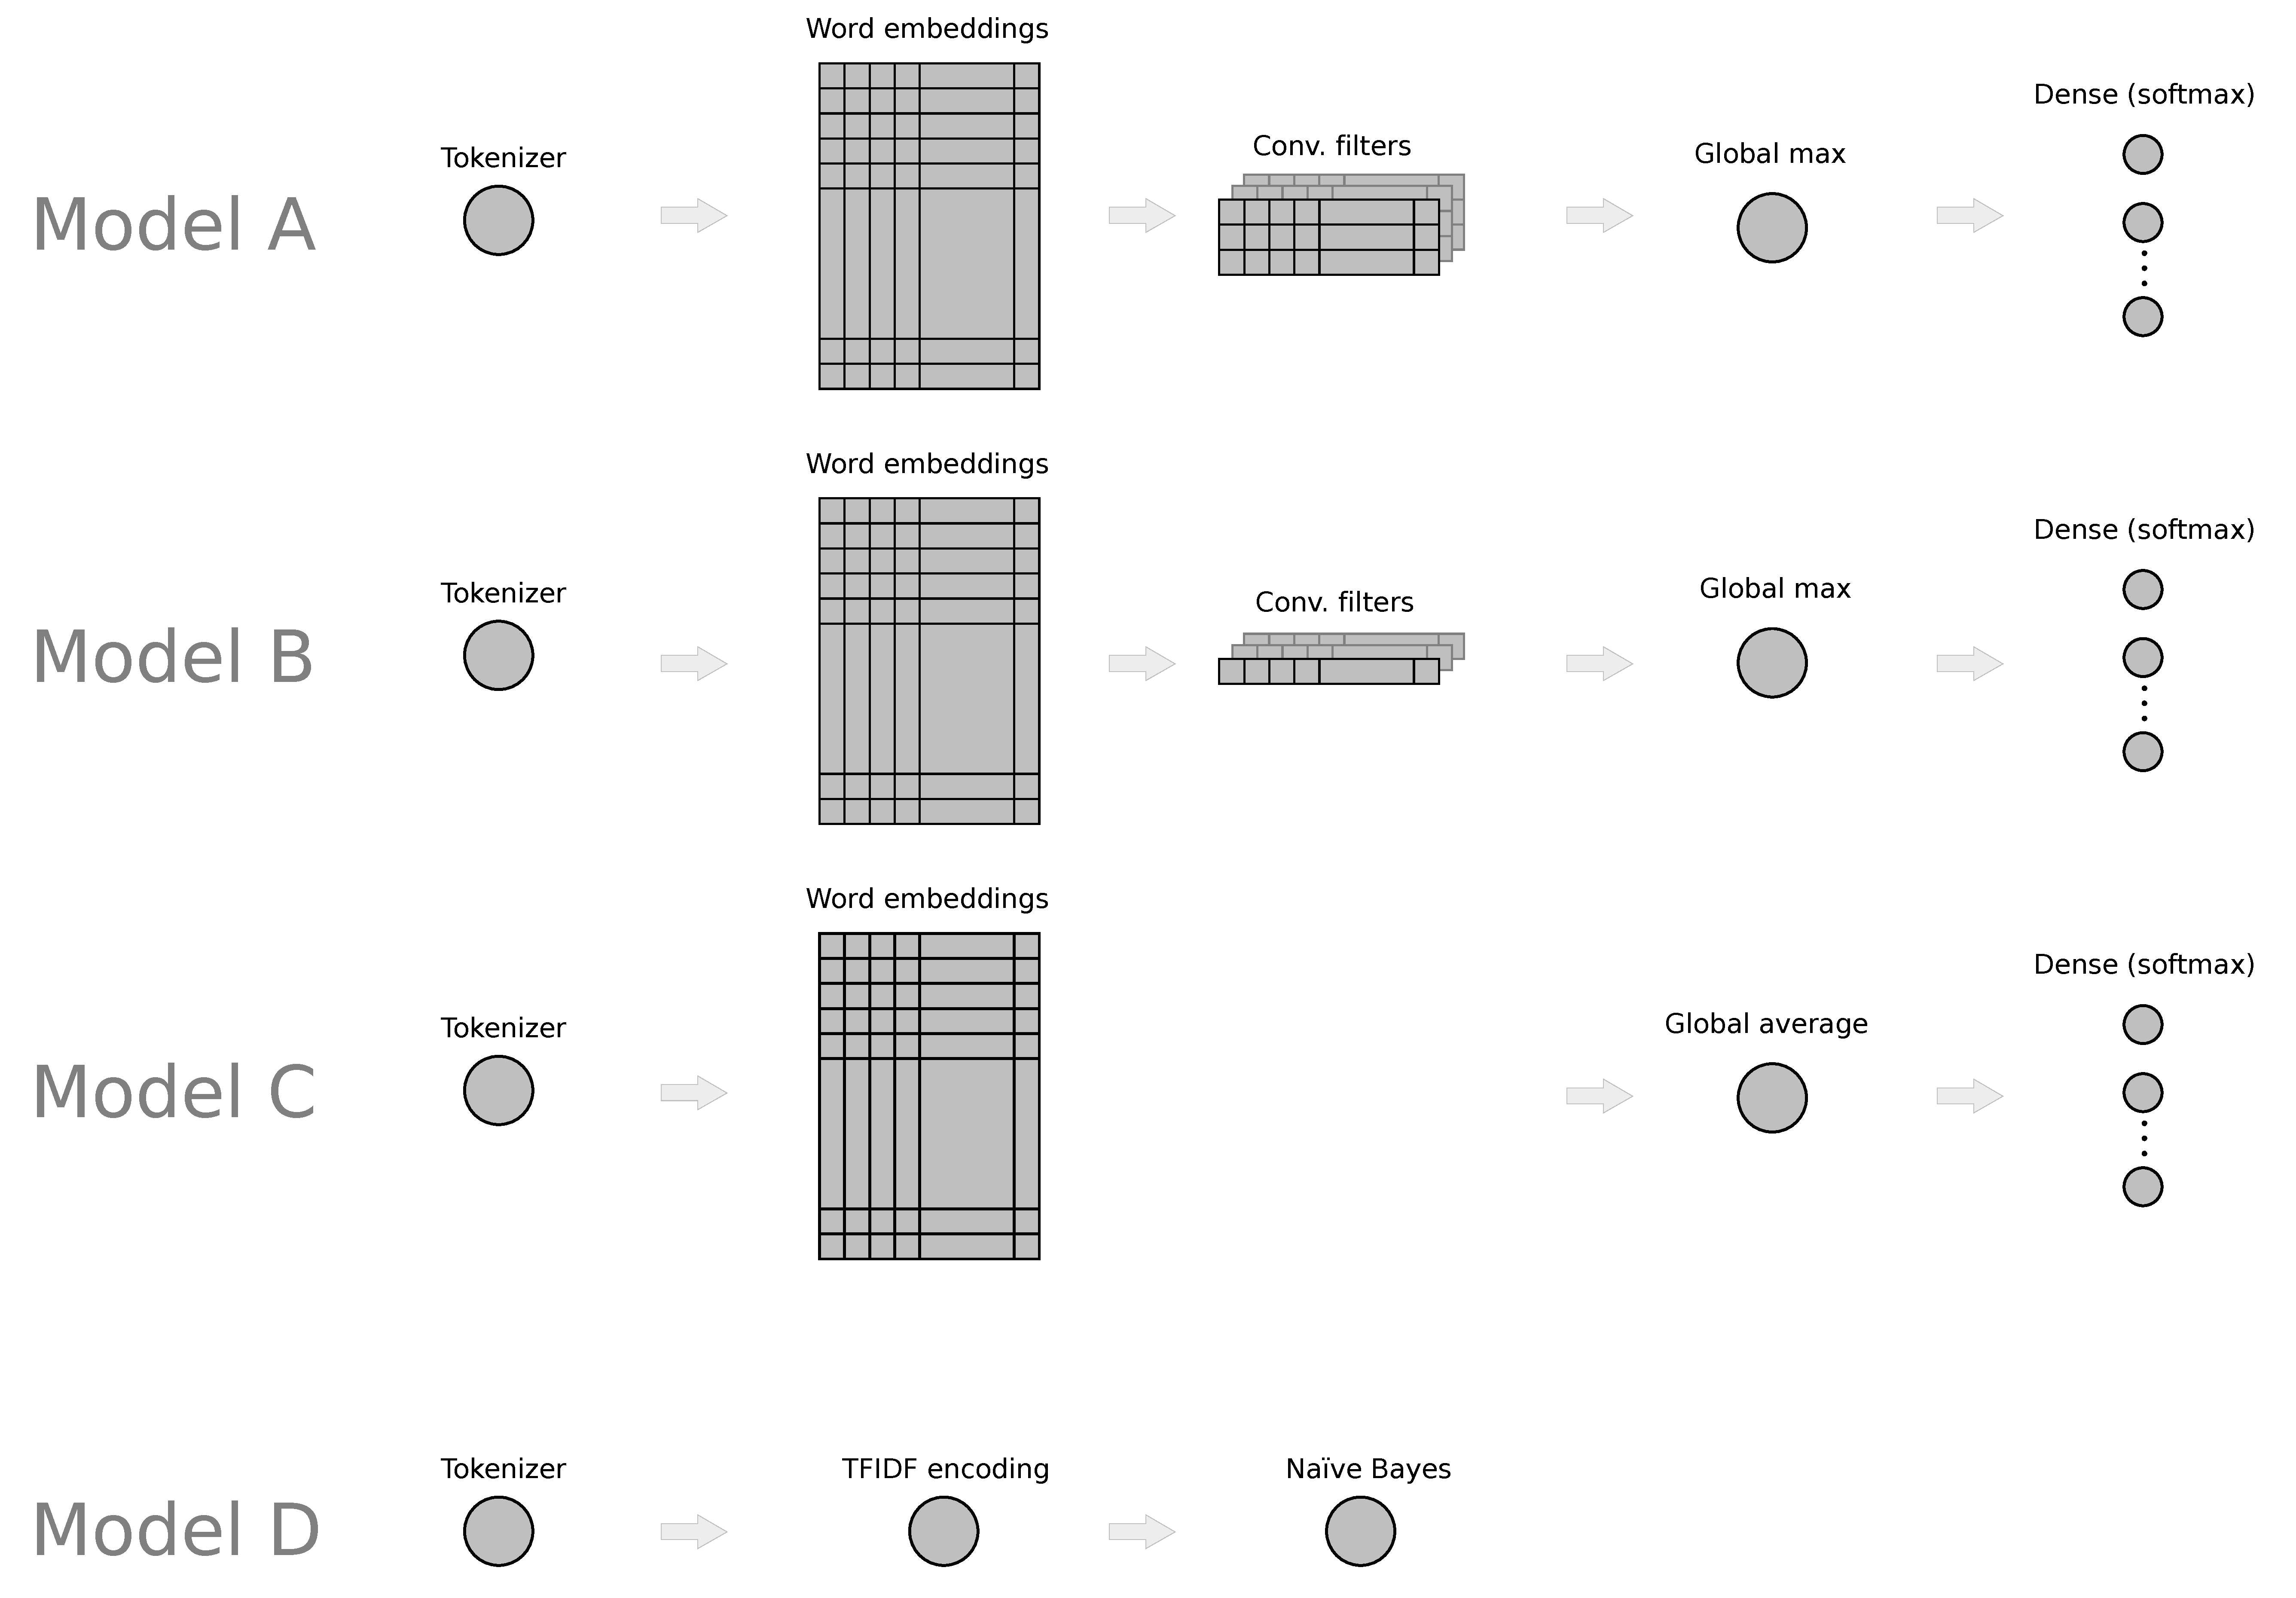
\includegraphics[width=\linewidth]{images/models01.pdf}
    \caption{Configurations of models A, B, C and D.}
    \label{fig:models}
\end{figure*}

\subsection{Metrics}

We assess the performance of all the models by calculating and comparing their \textit{accuracy}. We also use (validation) accuracy as the loss function when training our neural network models.

\begin{equation} 
\label{eq:accuracy}
    Accuracy = {TP + TN \over N}
\end{equation}

Where \textit{TP} is the number of true positives in the confusion matrix of the predictions for the test dataset, \textit{TN} the number of true negatives, and \textit{N} the total number of samples in the test split of the dataset.

In order to quantify how much relevant information we can additionally extract between models, we resort to calculate the \textit{information gain}. This magnitude, measured in bits, tells us how much more relevant information can a (better) model extract in comparison to another one. Following the design of the models explained above, we know that the only model that can extract positional information from text sequences is \textbf{Model A}, while both \textbf{Model B} and \textbf{Model C} can not. Thus, we assume we are able to estimate how good \textbf{Model A} in extracting such additional positional information, by comparing its results to those of \textbf{Model B} \textit{which we craft to be as similar as possible to Model A but preventing it from learning text sequence patterns}.

In order to calculate the \textit{information gain} between two models, we need to calculate first the \textit{entropy} of the original test dataset and also of the confusion matrices that result from applying the trained classifiers to the same dataset. 

The expression of \textit{entropy} for a multi-class dataset is:

\begin{equation}
    \label{eq:entropy1}
    H = - \sum_{i=1}^{N}  p_i \log_2(p_i)
\end{equation}

where $ p_i $ is the proportion or relative frequency of each class in the dataset and $ N $ the number of classes. In tune with this, the expression of the \textit{entropy (H)} for a set of samples that are classified with the same label is:

\begin{equation} 
\label{eq:entropy2}
    H(X|y \in Y) = - \sum_{x \in X} p(x|y) \log_2 p(x|y) 
\end{equation}

Where $ X = \{ x_1, x_2, ..., x_N\} $ is the set of real classes the documents belong to and $ Y $ the set of labels (i.e., to which classes the documents are assigned after classification). Thus, $ p(x|y) $ is the conditional probability that a document assigned to class \textit{y} after classification really belongs to class \textit{x}.

The resulting \textit{entropy} for the complete dataset after classification is the weighted average of the \textit{entropies} for each label:

\begin{equation} 
\label{eq:entropy3}
    H(X) = \sum_{y \in Y} p(y) \space H(X|y)
\end{equation}

Finally, the \textit{information gain} is calculated by subtracting the \textit{entropy} of the resulting classification for a model from the entropy of the (test) dataset.

\begin{equation} 
\label{eq:infogain1}
    IG(A) = H(X) - H_A(X)
\end{equation}

Where $ IG(A) $ is the \textit{information gain} that \textbf{Model A} gives over the test dataset. We can also consider \textit{information gain} between models:

\begin{equation} 
\label{eq:infogain2}
    IG(A,B) = H_B(X) - H_A(X)
\end{equation}

Where $ IG(A,B) $ is the \textit{information gain} that \textbf{Model A} gives over \textbf{model B}.

See \cite{Provost}, chapter 3, where this definition of \textit{information gain} is presented. Alternatively and equivalent to \textit{information gain}, we can calculate the \textit{mutual information} between predicted labels and real classes \cite{MI}:

\begin{equation} 
\label{eq:mutualinfo}
    I(X;Y) = \sum_{x \in X} \sum_{y \in Y} p(x,y) \log_2 \Big( {p(x,y) \over  p(x)p(y)} \Big)
\end{equation}

%%
%%
%%

\section{Analysis}
\subsection{Data Exploration}

We implement our model and analysis on the multi-class dataset \textit{20 Newsgroups} \cite{20Newsgroups}. This dataset can be directly imported from the Scikit-Learn \cite{Sklearn} library and comprises around 18000 newsgroups posts on 20 topics split in two subsets: one for training (development) and the other one for testing ( performance evaluation). The split between the train and test set is based upon messages posted before and after a specific date. The test split accounts for approximately the 40\% of the dataset. The exact proportions are summarized in Table \ref{tab:traintestsplit}.

\begin{table}[h]
\caption{20 Newsgroups dataset: number of documents per training and test dataset splits}
\label{tab:traintestsplit}
\begin{center}
\resizebox{.5\textwidth}{!}{%
    \begin{tabular}{||c|c|c||}
    \hline
    Number of documents & Training dataset & Test dataset \\
    \hline
    \hline
    18,846 & 11,314 & 7,532 \\
    \hline
    \end{tabular}
}
\end{center}
\end{table}

\subsubsection{Class distribution}

The 20 labels in the \textit{20 Newsgroups} dataset are the following:

\begin{multicols}{2}
\begin{enumerate}
    \item alt.atheism
    \item comp.graphics
    \item comp.os.ms-windows.misc
    \item comp.sys.ibm.pc.hardware
    \item comp.sys.mac.hardware
    \item comp.windows.x
    \item misc.forsale
    \item rec.autos
    \item rec.motorcycles
    \item rec.sport.baseball
    \item rec.sport.hockey
    \item sci.crypt
    \item sci.electronics
    \item sci.med
    \item sci.space
    \item soc.religion.christian
    \item talk.politics.guns
    \item talk.politics.mideast
    \item talk.politics.misc
    \item talk.religion.misc
\end{enumerate}
\end{multicols}

Quoting from \cite{20Newsgroups}, and referred to Table \ref{tab:groups}:

\say{
    Some of the newsgroups are very closely related to each other (e.g. comp.sys.ibm.pc.hardware / comp.sys.mac.hardware), while others are highly unrelated (e.g misc.forsale / soc.religion.christian). Here is a list of the 20 newsgroups, partitioned (more or less) according to subject matter: [...]
}

\begin{table*}[h]
\caption{20 Newsgroups dataset: grouped by content similarity}
\label{tab:groups}
\begin{center}
\resizebox{\textwidth}{!}{%
    \begin{tabular}{||l|l|l|l|l|l||}
    \hline
    Group A & Group B & Group C & Group D & Group E & Group F \\
    \hline
    \hline
    comp.graphics & rec.autos & sci.crypt & misc.forsale & talk.politics.misc & talk. religion.misc \\
    comp.os.ms-windows.misc & rec.motorcycles & sci.electronics & & talk.politics.guns & alt.atheism \\
    comp.sys.ibm.pc.hardware & rec.sport.baseball & sci.med & & talk.politics.mideast & soc.religion.christian \\
    comp.sys.mac.hardware & rec.sport.hockey & sci.space & & & \\
    comp.windows.x & & & & & \\
    \hline
    \end{tabular}
}
\end{center}
\end{table*}

\begin{figure}[h]
      \centering
      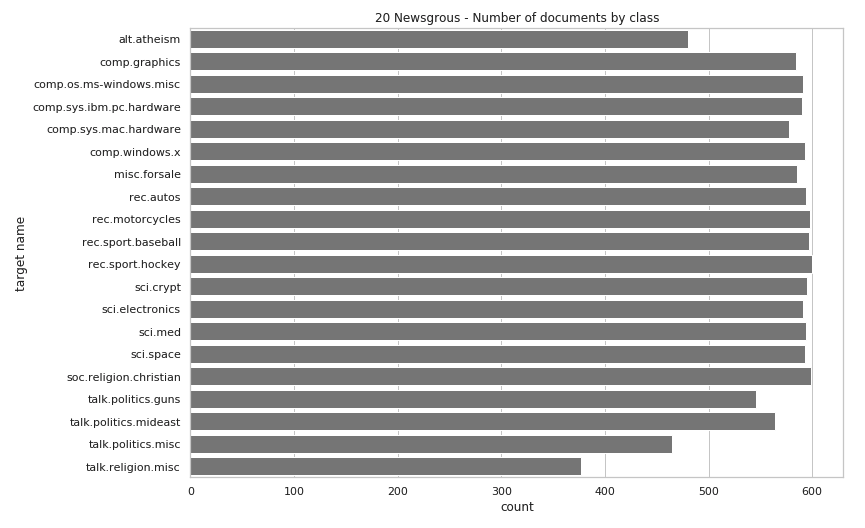
\includegraphics[width=\linewidth]{images/chart_01.png}
      \caption{20 Newsgroups - Number of documents by class (training split). Entropy = 4.314 bits}
      \label{fig:numbyclass}
\end{figure}

The proportion of documents by class is displayed in Figure \ref{fig:numbyclass}. According to the dataset distribution of classes and Equation \ref{eq:entropy1}, the \textbf{entropy of the dataset} is \textbf{4.314 bits}, both for the training and test divisions. The entropy for a perfectly balanced dataset of 20 classes would be 4.322 bits, less than 0.2\% away from the entropy of our dataset. Thus, we can say we have a fairly \textit{balanced dataset in terms of class distribution}.

\subsubsection{Document structure}

The content of the documents is that of an e-mail. Thus, in addition to the body of the message, we have a header, and possibly footer and inline quotes. As pointed out in the the Scikit-learn documentation \cite{Sklearn}, headers, footers and quotes make the classifier to easily overfit and learn helpful patterns that do not reside in the body of the message. For that reason, we will remove them. Quote from Scikit-learn documentation:

\say{
    When evaluating text classifiers on the 20 Newsgroups data, you should strip newsgroup-related metadata. In scikit-learn, you can do this by setting remove=('headers', 'footers', 'quotes'). The F-score will be lower because it is more realistic.
}

\begin{figure*}[h]
\caption{A document from our dataset}
\begin{verbatim}
From: mwbg9715@uxa.cso.uiuc.edu (Mark Wayne Blunier)
Subject: Re: 5W30, 10W40, or 20W50
Organization: University of Illinois at Urbana
Lines: 12

zowie@daedalus.stanford.edu (Craig "Powderkeg" DeForest) writes:

>If you're planning on making long drives, the 20W50 is probably fine
>(esp. in the summer) in your 10W40 car.  But if you're making short drives,
>stick to the 10W40.

Several years ago GM was having trouble with the rings sticking on the
5.7 diesel.  They traced a cause to the use of 10W-40 oil.  They would
not honor warranty work if 10W-40 was used (if my memory serves me).
5-30, 10-30 or 20 50 was OK'd though.

Mark B.
\end{verbatim}
\label{doc1}
\end{figure*}

\begin{figure*}[h]
\caption{The document from our dataset shown in Figure \ref{doc1}, without headers, footers and quotes}
\begin{verbatim}
Several years ago GM was having trouble with the rings sticking on the
5.7 diesel.  They traced a cause to the use of 10W-40 oil.  They would
not honor warranty work if 10W-40 was used (if my memory serves me).
5-30, 10-30 or 20 50 was OK'd though.
\end{verbatim}
\label{doc2}
\end{figure*}

In Figure \ref{doc1} a document from the training set, index=201, is shown. The same document with headers, footers and quotes removed, in Figure \ref{doc2}.

\subsubsection{Text length distribution}

Document length statistics for the training, test and combined datasets are shown in Table \ref{tab:doclength}.  In Figure \ref{fig:doclength} we use a \textbf{letter-value plot} \cite{letter-value-plot} to depict length distribution of both training and test datasets. We find this kind of visualization to be a better option to spot outliers in our dataset than Tukey's box-plot. As stated in \cite{letter-value-plot}: 

\say{
    Larger data sets (n $\approx $  10,000-100,000) afford more precise estimates of quantiles beyond the quartiles, but conventional boxplots do not show this information about the tails, and, in addition, show large numbers of extreme, but not unexpected, observations.
}

From Figure \ref{fig:doclength} we notice 20 outliers in the training dataset, all of them longer than 10,000 tokens. We carried out visual inspection of each of them and found out that three of them were transcriptions of long documents while the other 17 were multi-part multimedia embedded messages. As the proportion of these kind of documents is very small, we preferred to preserve the integrity of the dataset and not perform any kind of document removal.

\begin{table}[h]
\caption{Document length statistics (num. of tokens)}
\label{tab:doclength}
\begin{center}
\resizebox{.8\textwidth}{!}{%
    \begin{tabular}{||c|c|c|c|c|c|c|c|c|c||}
    \hline
    Dataset split & entropy (bits) & count (docs) & mean & std & min & 25\% & 50\% & 75\% & max \\
    \hline
    \hline
    Train & 4.314 & 11314 & 210.5 & 778.5 & 0 & 41.0 & 85.0 & 169.0 & 16306 \\
    Test & 4.314 & 7532 & 179.1 & 583.2 & 0 & 39.0 & 81.0 & 162.0 & 28592 \\
    Combined & 4.314 & 18846 & 198.0 & 707.1 & 0 & 40.0 & 83.0 & 167.0 & 28592 \\
    \hline
    \end{tabular}
}
\end{center}
\end{table}

\begin{figure*}[h]
      \centering
      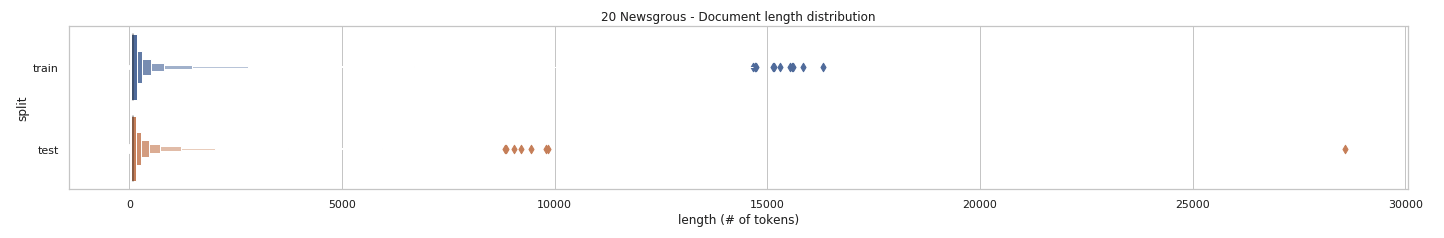
\includegraphics[width=\linewidth]{images/chart_06.png}
      \caption{20 Newsgroups - Document length distribution}
      \label{fig:doclength}
\end{figure*}

\subsubsection{Conclusions about the dataset}

Our dataset is a well-known example of multi-class classification, with a fairly high number of classes (20). While classes are very balanced in terms of proportions, document lengths vary a lot, from empty documents to 28,592 tokens, approximate mean of 198 tokens, and a large standard deviation of 707 tokens. In our investigation we need to consider a maximum length to truncate the documents so that they retain enough information for the classification purpose but they do not overload the expensive computation that is required to train the CNN. The chosen length we decide to truncate documents to is \textit{1,000 tokens}, as only a fairly small proportion, \textit{only 2.4\% of the documents of the training dataset, are longer}. 

%%
%%
%%
% \subsection{Exploratory Visualisation}

%%
%%
%%
\subsection{Algorithms and Techniques}

As mentioned, we built four models. We describe them in more detail now.

\subsubsection{Models}

\begin{figure*}[p]
    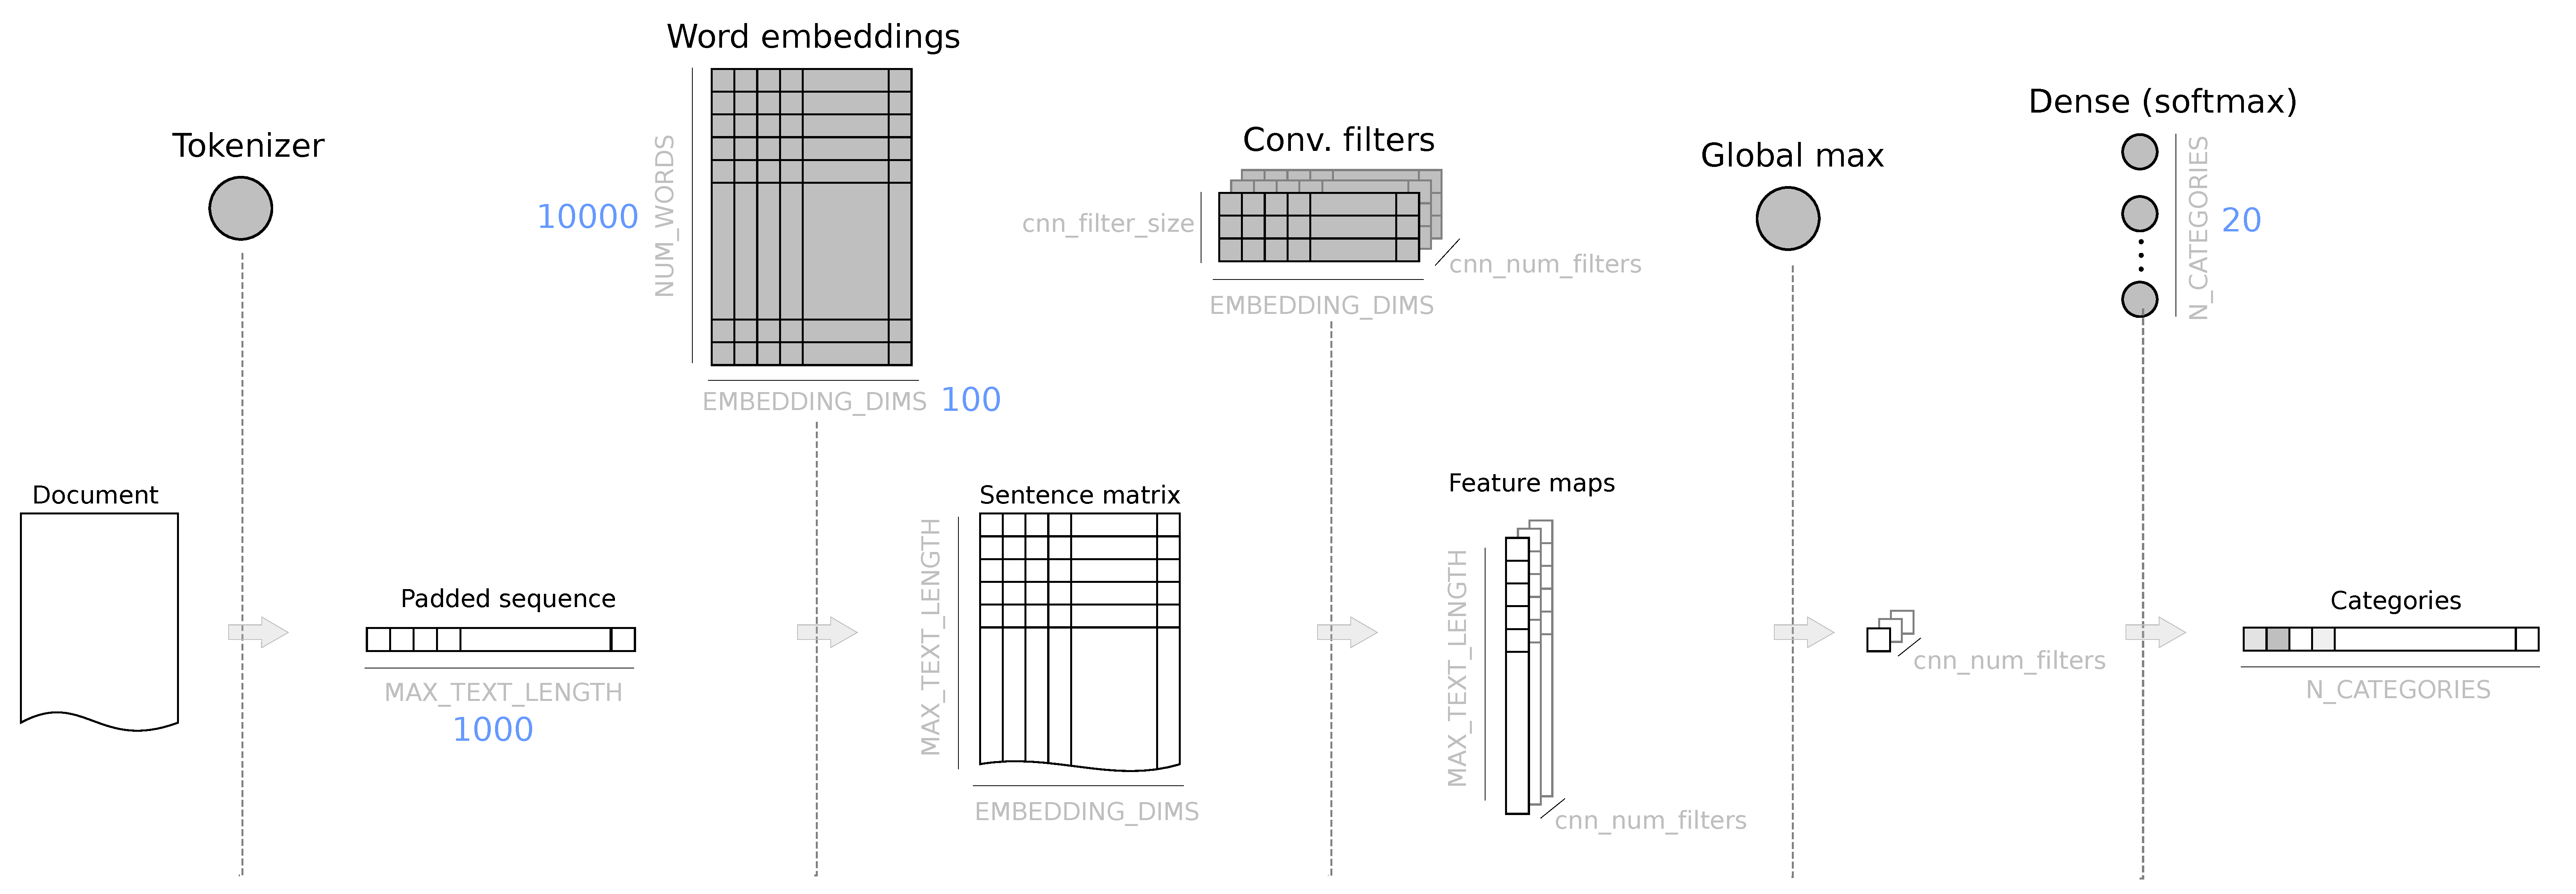
\includegraphics[width=\linewidth]{images/models02.pdf}
    \caption{Model A}
    \label{fig:modelA}
\end{figure*}
\begin{figure*}[p]
    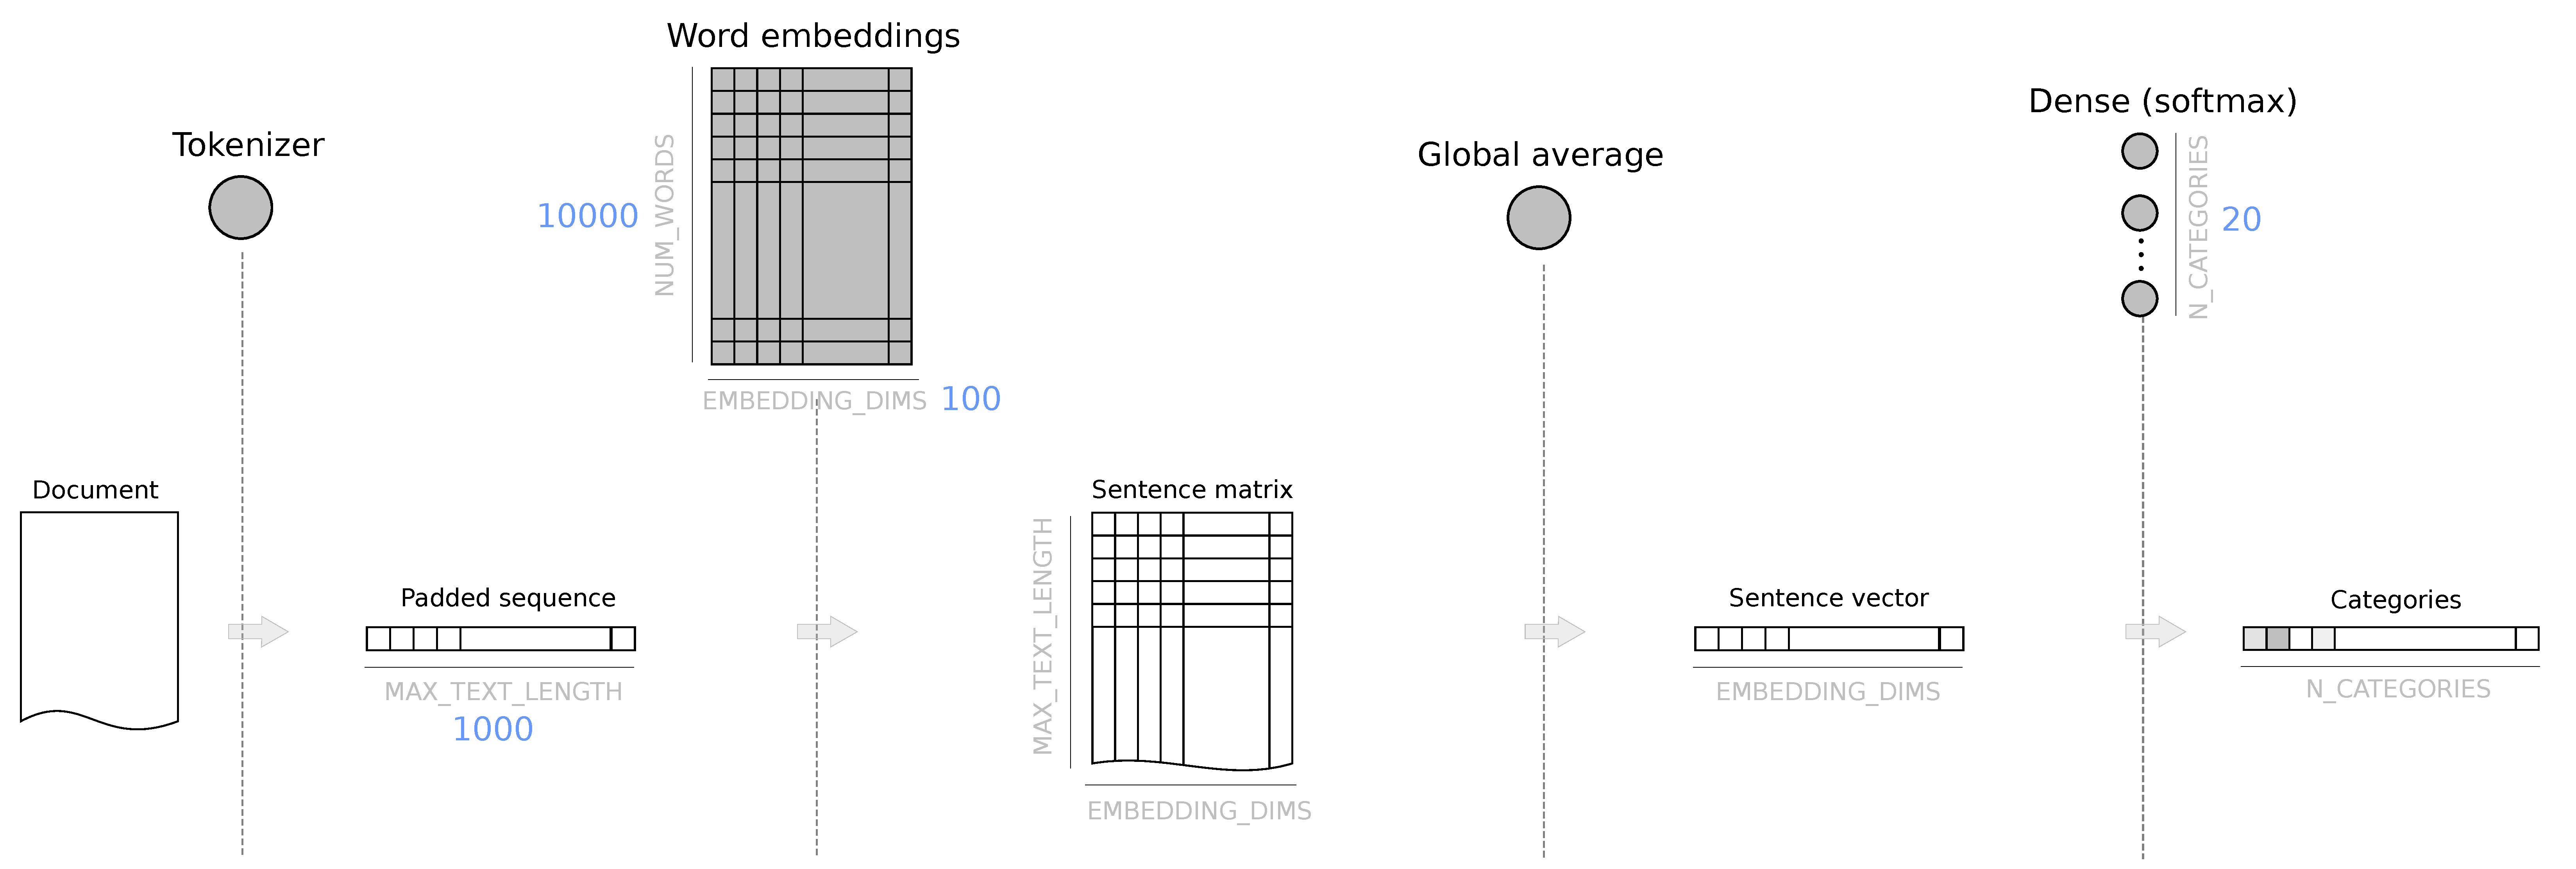
\includegraphics[width=\linewidth]{images/models03.pdf}
    \caption{Model C}
    \label{fig:modelC}
\end{figure*}
\begin{figure*}[p]
    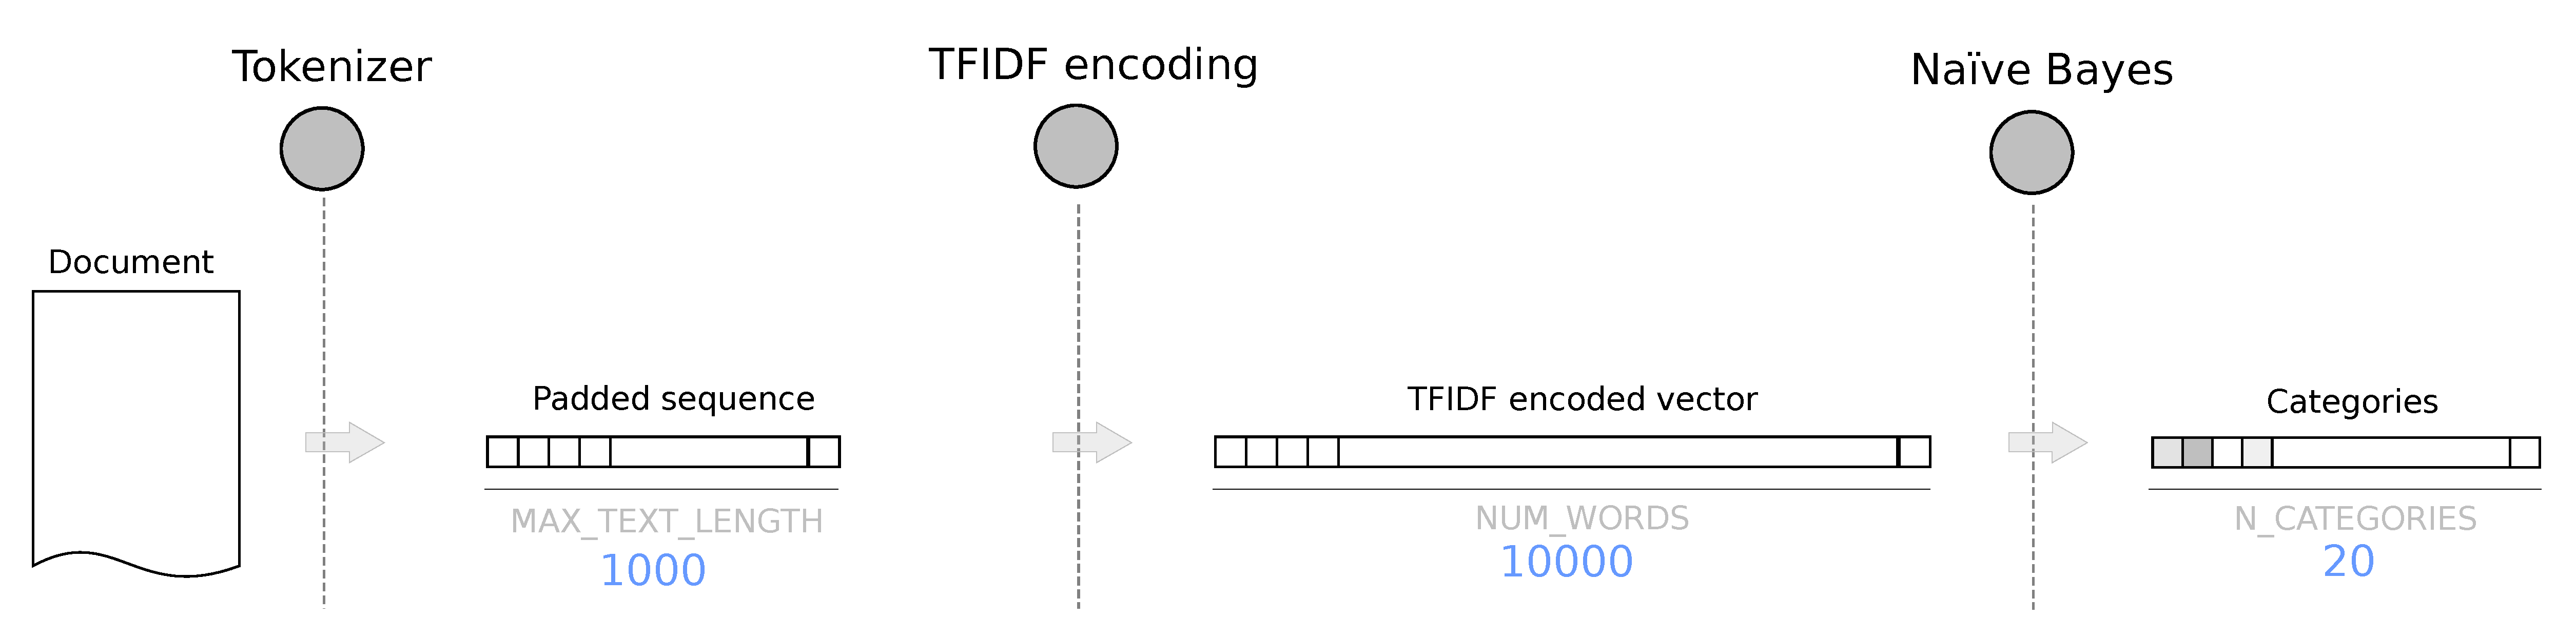
\includegraphics[width=\linewidth]{images/models04.pdf}
    \caption{Model D}
    \label{fig:modelD}
\end{figure*}

\textbf{Model A} is displayed in figure \ref{fig:modelA}. Its first layer  is a \emph{tokenizer}, which converts each text document into sequences of integers where each number represents a word in a dictionary that contains all the words that are present in the corpus. The next layer, \emph{embeddings}, converts each number within a sequence into a dense vector of 100 dimensions. The output is then a sequence matrix which has as many rows as tokens in the document and as many columns as dimensions in the embeddings representation. Then, a \emph{convolutional layer} of dimension 1 is applied to the sequence matrix. The size of the filters is the main hyper-parameter to explore, from 2 to 9, trying to detect which size is able to achieve better classification results. We also explore the best number of filters to use in this convolutional layer. The outcome of this stage is a set of \emph{feature maps}, one per filter, each one being a sequence of values with same length as the original text sequences. After that, a \emph{global max. pooling layer} reduces each feature map to a single value. All these values coming from reducing feature maps are then concatenated to form a vector of length equal to the number of filters. Finally, a \emph{dense neural net layer} of 20 nodes with softmax activation function and some regularization  (dropout and norm constraint) is applied to get the final array of 20 values which represent the probabilities the document has to belong to each one of the 20 categories of the dataset. 

We follow the guidelines in \cite{Zhang} for this type of CNN architecture and use the same recommended starting values for model hyperparameters, shown in Table \ref{tab:hparams}, although with a couple of changes:

\begin{itemize}
    \item Instead of \textit{word2vec}, we use \textit{GloVe} embeddings.
    \item In \cite{Zhang} they propose 3 parallel channels in the convolutional layer, with 3 different consecutive filter sizes. We simplify the architecture by using a single convolutional channel with a unique CNN filter size; and in order to compensate model complexity and pattern recognition power, we multiply by 3 the number of feature maps we use as starting point.
\end{itemize}


\begin{table}[h]
\caption{Starting hyperparameters for Model A}
\label{tab:hparams}
\begin{center}
\resizebox{.6\textwidth}{!}{%
    \begin{tabular}{|l|l|l|}
    \hline
    Description & Values suggested in \cite{Zhang} & Used values \\
    \hline
    \hline
    input word vectors & Google word2vec \cite{word2vec}& \textbf{GloVe} \cite{Pennington} \\
    filter region size & (3,4,5) & \textbf{4} \\
    feature maps & 100 &    \textbf{300} \\
    activation function & ReLU & ReLU \\
    pooling & 1-max pooling & 1-max pooling \\
    dropout rate & 0.5 & 0.5 \\
    l2 norm constraned & 3 & 3 \\
    \hline
    \end{tabular}
}
\end{center}
\end{table}


\textbf{Model B} is the result of modifying \textbf{Model A} by setting the convolutional filter size to 1. \textbf{Model C}, displayed in figure \ref{fig:modelC}, is the result of modifying Model A by removing the convolutional layer and substituting the global max. pooling layer by a global average layer. \textbf{Model D}, depicted in figure \ref{fig:modelD}, is the baseline benchmark model, which is based on a Multinomial Naïve Bayes classifier applied on a TFIDF (Term Frequency - Inverse Document Frequency) representation of each document. 

\subsubsection{Libraries}

In order to implement, train and evaluate our models, we used Python 3 and two main libraries:

\begin{itemize}
    \item \textbf{Keras} \cite{Keras}, used to implement the neural network models (A, B and C) and also to pre-process the dataset (tokenizer).
    \item \textbf{Scikit-Learn} \cite{Sklearn}, used to load the \textit{20 Newsgroups} dataset and also to implement the baseline model (Naïve Bayes classifier).
\end{itemize}

\subsubsection{Computing environment}
Due to the high demand of processing resources associated to training deep neural networks, we wrote and executed our code in \textbf{Google Colab} using a notebook connected to a GPU-enabled python kernel. 


\subsection{Benchmark}
Our benchmarking strategy is based on comparing the scores we get for the 4 proposed models.

\begin{itemize}
    \item \textit{Accuracy}. We compare the final accuracy of models A, B, C and D on the test dataset. 
    \item \textit{Information Gain}. We assess the \textit{information gain} of each model in comparison with the \emph{entropy} of the test dataset. This is equivalent to calculating the \textit{mutual information} of the resulting classification (i.e., of the confusion matrix after evaluating each model on the test dataset).
\end{itemize}

Our initial assumption is that models A, B and C should be significantly better than Model C regarding \textit{accuracy} and \textit{information gain}, as their complexity is much higher. On top of this, if scores for Model A turned out to be significantly better than for Model B, then we would have some basis to say that Model A is managing to extract some additional \emph{positional} information from the dataset, as the latter was conceived to be as similar to the former as possible except for the fact that, due to its convolutional filters of length 1,  it cannot extract positional information. Finally, evaluating Model C and comparing it to Model B could give us a measure of how much good a convolutional layer does when extracting non-positional information compared to the contributions of the embeddings and dense layers.

%%
%%
%%
\section{Methodology}
\subsection{Data Preprocessing}

\subsubsection{Load dataset}
The \textit{20 Newsgroups} dataset was loaded by using the utility function \verb|fetch_20newsgroups| provided by the Scikit-learn library, both for the training and test splits. We removed headers, footers and quotes by specifying the parameter \verb|remove| of the \verb|fetch_20newsgroups| function:

\begin{lstlisting}[language=Python]
from sklearn.datasets import fetch_20newsgroups
dataset_train = fetch_20newsgroups(subset='train', remove=('headers', 'footers', 'quotes'))
\end{lstlisting}

\subsubsection{Document tokenization}\label{sec:tokenization}
The next step was tokenizing the documents in the corpus. For that purpose we used the \verb|Tokenizer| class in the Keras library. In the tokenizing process we considered only the \textbf{10,000 most common words} in the dataset. Then, we built several matrices that worked as inputs and target outputs for our models:

\begin{itemize}
    \item \verb|X_tfidf_train|. Each row in this matrix represents a document in the training dataset, encoded with the TFIDF method. Each column represents a word in the set of 10,000 most common words in the dataset.
    \item \verb|X_tfidf_test|. Same as above but for the test dataset.
    \item \verb|X_seqs_train|. Each row represents a document in the training dataset, encoded as a sequence of integers (each value corresponds to a word in the set of most common 10,000 words). In order to have constant length rows, these sequences were padded with zeros on the left, and truncated to the \textbf{maximum length of 1,000 words}.
    \item \verb|X_tfidf_test|. Same as above but for the test dataset.
    \item \verb|Y_train|. Matrix of integers that represents the labels (classes) for each document in the training dataset.
    \item \verb|Y_test|. Same as above but for the test dataset.
    \item \verb|Y_1hot_train|, \verb|Y_1hot_test|. 1-hot encoding representation of both label matrices above, needed for calculating categorical cross-entropy (loss) when training and evaluating the neural network models.
\end{itemize}

\subsubsection{Word embeddings layer}
We downloaded the \textit{GloVe} pre-trained word vectors \cite{Pennington} from \textit{GloVe: Global Vectors for Word Representation} web page: \url{https://nlp.stanford.edu/projects/glove/}. Details of the file: Wikipedia 2014 + Gigaword 5 (6B tokens, 400K vocab, uncased, 50d, 100d, 200d \& 300d vectors, 822 MB download). We took the vector representation that use \textbf{100 dimensions} and built an embedding matrix that was to pre-loaded in our neural network models (A, B and C).

\begin{table}[h]
    \centering
    \resizebox{.8\textwidth}{!}{%
    \begin{tabular}{||l | r | l ||}
        \hline
        Parameter & Value & Description \\
         \hline
         \hline
         \verb|NUM\_WORDS & 10,000 & Num. of most common words in tokenization and embeddings \\
         \verb|MAX\_TEXT\_LENGTH & 1,000 & Max. length documents are truncated to\\
         \verb|EMBEDDING\_DIMS & 100 & Num. of dimensions of embeddings  \\
         \hline
    \end{tabular}
    }
    \caption{Fixed model parameters}
    \label{tab:fixedparams}
\end{table}

\subsection{Implementation}\label{sec:implementation}

The implementation process followed these steps:

\begin{enumerate}
    \item Hyperparameter exploration and training of \textbf{Model A}
    \item Training of \textbf{Model B} (inheriting best hyperparamter values from Model A)
    \item Training of \textbf{Model C} (inheriting best hyperparamter values from Model A)
    \item Hyperparameter exploration and training of \textbf{Model D}
    \item Evaluation of models and score comparison
\end{enumerate}

\subsubsection{Hyperparameter exploration and training of Model A}\label{sec:trainingmodelA}

\begin{table}[h]
    \centering
    \resizebox{\textwidth}{!}{%
    \begin{tabular}{||c | c | c | c ||}
        \hline
        Hyperparameter & Description & Explored values & Exploration phase \\
         \hline
         \hline
         \verb|optimizer & optimizer &  rmsprop, adagrad, adam, nadam & 0 \\
         \verb|batch\_size & batch size & 64,128,256,512  &\\
         \hline
         \verb|embedding\_preload & preload \textit{GloVe} embeddings & True, False & 1 \\
         \verb|embedding\_train & train embeddings layer & True, False &  \\
         \hline
         \verb|cnn\_filter\_size & CNN filter size (filter region size) & 2,3,4,5,6,7,8,9 & 2 \\
         \verb|cnn\_num\_filters & num. convolutional filters (feature maps) & 100,300,600,900 & \\
         \hline
    \end{tabular}
    }
    \caption{Hyperparameter exploration for Model A}
    \label{tab:explorationgrid}
\end{table}

Table \ref{tab:explorationgrid} shows the hyperparameters and values we explored when training Model A. According to this table, we considered 6 hyperparameters and a total of 2048 combinations, an overwhelming number for a neural network to be trained even with the support of GPUs. Thus, we decided to divide the exploration in three phases. Keeping in mind that the most relevant hyperparamters in our investigation are \textit{convolutional filter size} and \textit{number of convolutional filters}, we left the exploration of these two to the final phase. In each phase we performed a grid search only for two selected hyperparameters, as follows:

\begin{enumerate}
    \item First, we tried to find the best hyperparameter values for \textit{batch size} and \textit{optimizer type}, leaving the rest of hyperparameters fixed to the values suggested as starting point in Table \ref{tab:hparams}. We performed a grid search and trained Model A with all the hyperparameter combinations shown for this phase in Table \ref{tab:explorationgrid}. We picked the best combination according to the best \textit{validation accuracy} obtained in the process. 
    \item Then, we fixed the best values we found for \textit{batch size} and \textit{optimizer type} and explored the effect of preloading the embedding layer with the GloVe word vectors, and if the weights of the embedding layer should be optimised during training or left as they had been pre-loaded. Again, we trained Model A with the 4 combinations and selected the best one according to the best validation accuracy.
    \item After that, we fixed the values for both hyperparameters \textit{embedding preload} and \textit{embedding train} and then explored the \textit{convolutional filter size} and \textit{number of filters} in the convolutional layer. We scanned values from 2 to 10 for the convolutional filter size, and tried number of filters 100, 300, 600 and 900.
\end{enumerate}

After the exploration process we had found a final combination of hyperparameters from all the possibilities shown in Table \ref{tab:explorationgrid}, and could finally train Model A with it. We saved the best found configuration for Model A and the computed model weights so that we could recreate a trained instance of the model without further training.

\subsubsection{Training Model B}

We created then an instance of Model B by inheriting the best combination of  hyperparameters from Model A, but changing the value of \textit{convolutional filter size} to 1. As explained, we wanted to force the new model not to be able to extract positional information from the text sequences while being very similar to Model A. We trained this instance of Model B and also saved the resulting weights.

\subsubsection{Training Model C}

In a similar way, we created a new instance of a neural network, but this time by modifying Model A and removing the convolutional layer and substituting the \textit{global max pooling layer} with a \textit{global average pooling layer} (figure \ref{fig:modelC}). Again, we re-used the best hyperparameter values we found for Model A except for \textit{convolutional filter size} and \textit{number of convolutional filters}, which were not applicable anymore. We trained this instance of Model C to get and save its weights.


\subsubsection{Number of epochs}

While carrying out the hyperparameter exploration process to pick the best hyperparamter combinations we always used the same number of epochs, 20, in order to train the convolutional neural net. We wanted to keep it to a small value to save computing resources and time. However, once the hyperparamter selection was done and we went on to training the final instances of models A, B and C, we had to check in each case if the number of epochs was enough for the validation accuracy to reach a stable \textit{plateau} through epochs (Figure \ref{fig:epochs}). Considering this, we decided to train models A and B along 30 epochs, and we had to increase that value to 1,000 epochs for Model D. 

\begin{figure*}[h]
\begin{tabular}{c c}
    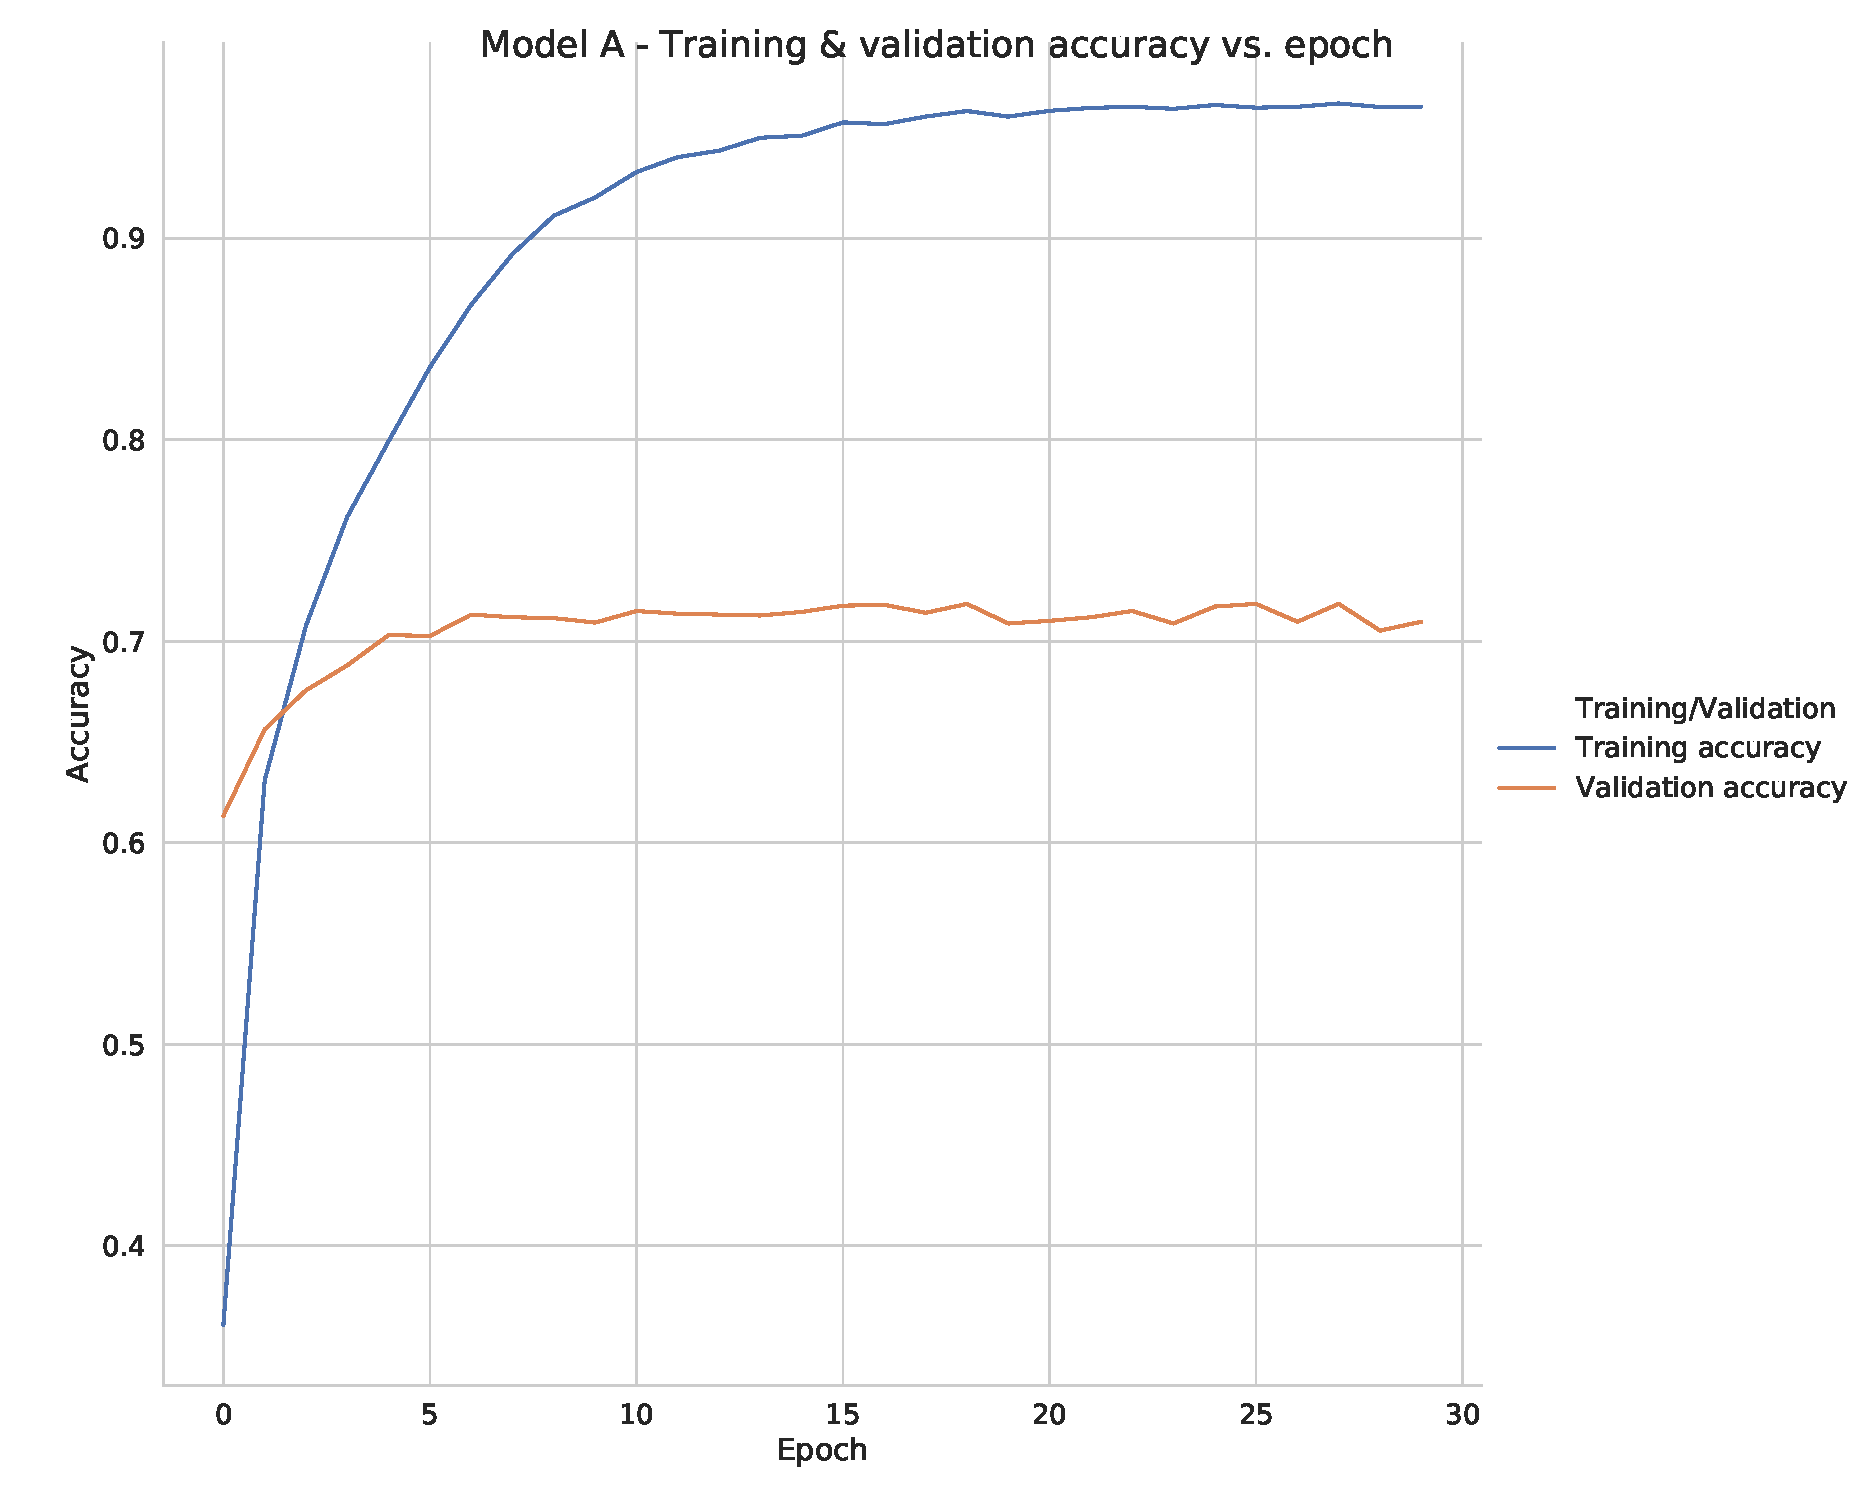
\includegraphics[width=.502\linewidth]{images/chart_16.pdf} &
    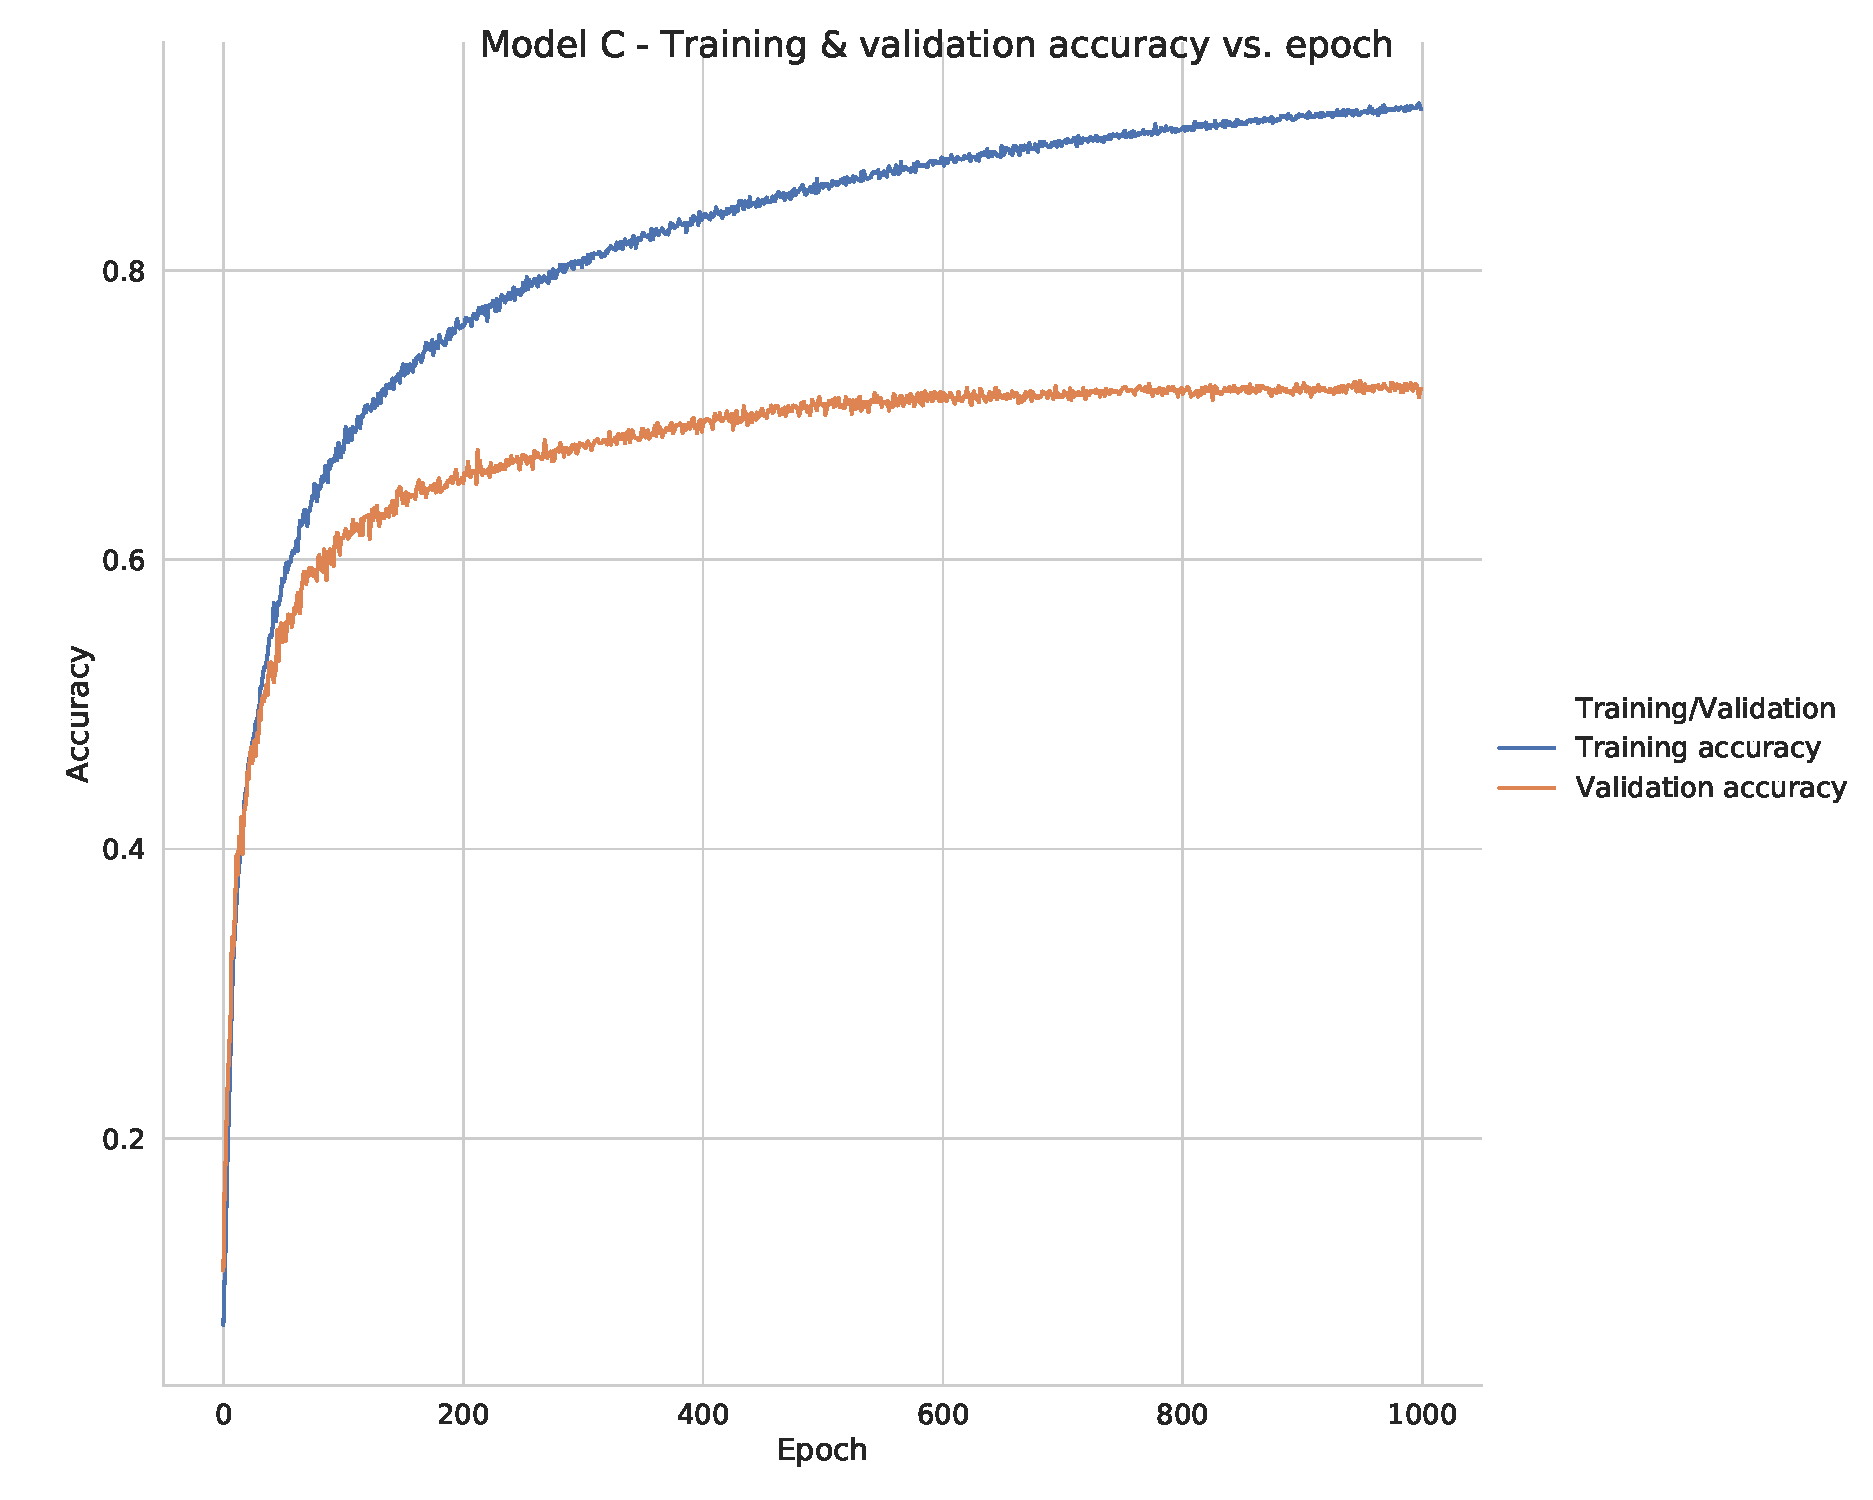
\includegraphics[width=.498\linewidth]{images/chart_18.pdf} \\
\end{tabular}
\caption{Validation and training accuracy along epochs for models A and C, configured with hyperparameters in figure \ref{tab:besthyperparams}}
\label{fig:epochs}
\end{figure*}

\subsubsection{Hyperparameter exploration and training of Model D}

Finally, we trained the baseline benchmark model, a Multinomial Naïve Bayes classifier applied on TFIDF document representations. The simplicity of the model led us to only explore hyperparameter \textit{alpha} (additive Laplace/Lidstone smoothing parameter \cite{Sklearn}) from 0.1 to 1.0 in 0.1 steps. The model trains and runs pretty fast so we decided not to save its trained weights in a file.

\subsubsection{Model evaluation}

After hyperparameter exploration and model training, we went on to model evaluation. We created new fresh model instances with the hyperparamter values that resulted from our exploration process. We loaded the serialized weights from files into each model instance. Then, we proceeded to calculate the scores \textit{accuracy} and \textit{information gain} for each model. In order to calculate accuracies we did the following:

\begin{itemize}
    \item For models A, B and C (based on Keras) we applied the Keras method \verb|model.evaluate(X_seqs_test, Y_1hot_test)|. Refer to matrix definitions in \ref{sec:tokenization}.
    \item For Model C (based on Scikit-learn) we applied the Scikit-learn method \verb|model.score(X_tfidf_test, Y_test)|. 
\end{itemize}

In both cases, and "under the hood", the model was applied to obtain prediction matrices, counts of true positives and true negatives were carried out and, after that, Equation \ref{eq:accuracy} was applied. Then, for calculating the \textit{information gain} we followed these steps:

\begin{enumerate}
    \item We applied each model to the input matrix for the test dataset (\verb|X_seqs_test| for models A, B and C; \verb|X_tfidf_test| in the case of model D). The predicted values were converted from 1-hot to categorical encoding and stored in matrices \verb|Y_predictionA|,  \verb|Y_predictionB|, \verb|Y_predictionC|, and \verb|Y_predictionD|.
    \item From these output matrices we calculated the corresponding confusion matrices by applying the Scikit-learn function \verb|confusion_matrix(Y_test, Y_prediction)|. See a sample of the confusion matrices for our 4 models visualized in figure \ref{fig:confusionmatrix}.
    \item From the confusion matrices, we calculated the \textit{information gain} using Equation \ref{eq:infogain1} (alternatively and equivalently the \textit{mutual information}, Equation \ref{eq:mutualinfo}, can be used).
\end{enumerate}


\begin{figure*}[h]
\begin{tabular}{c c}
    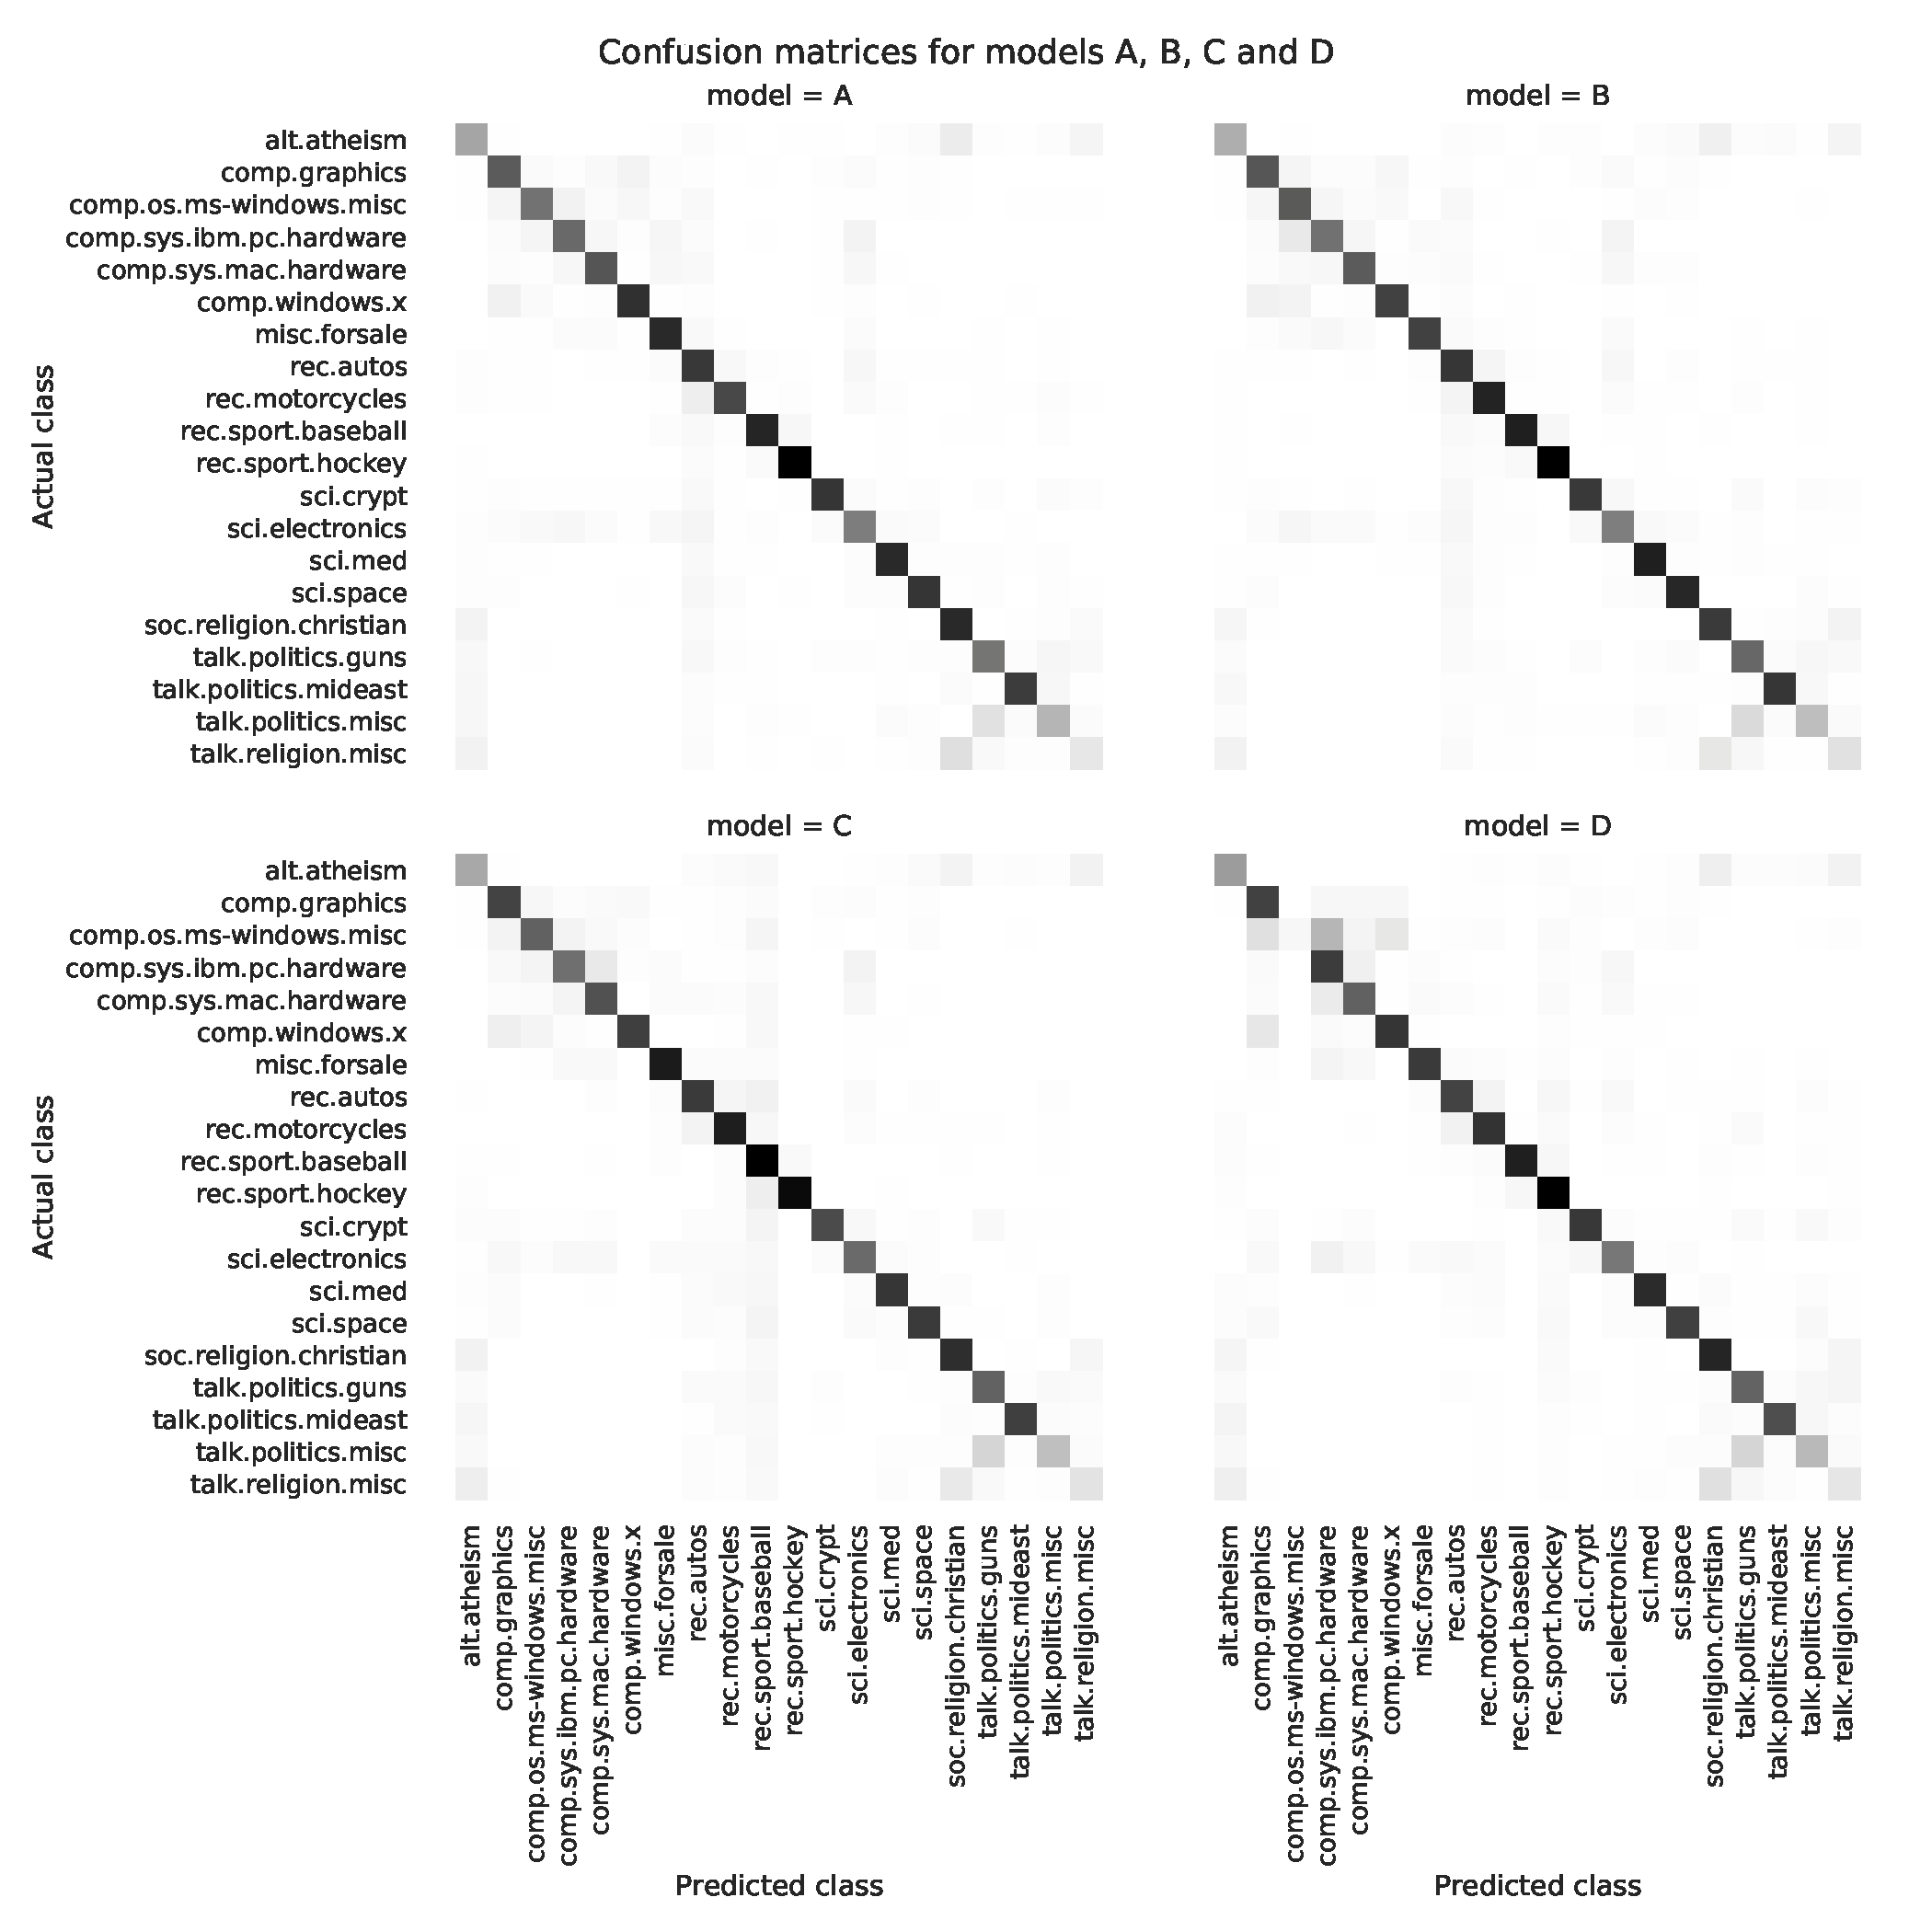
\includegraphics[width=.50\linewidth]{images/chart_20.pdf} &
    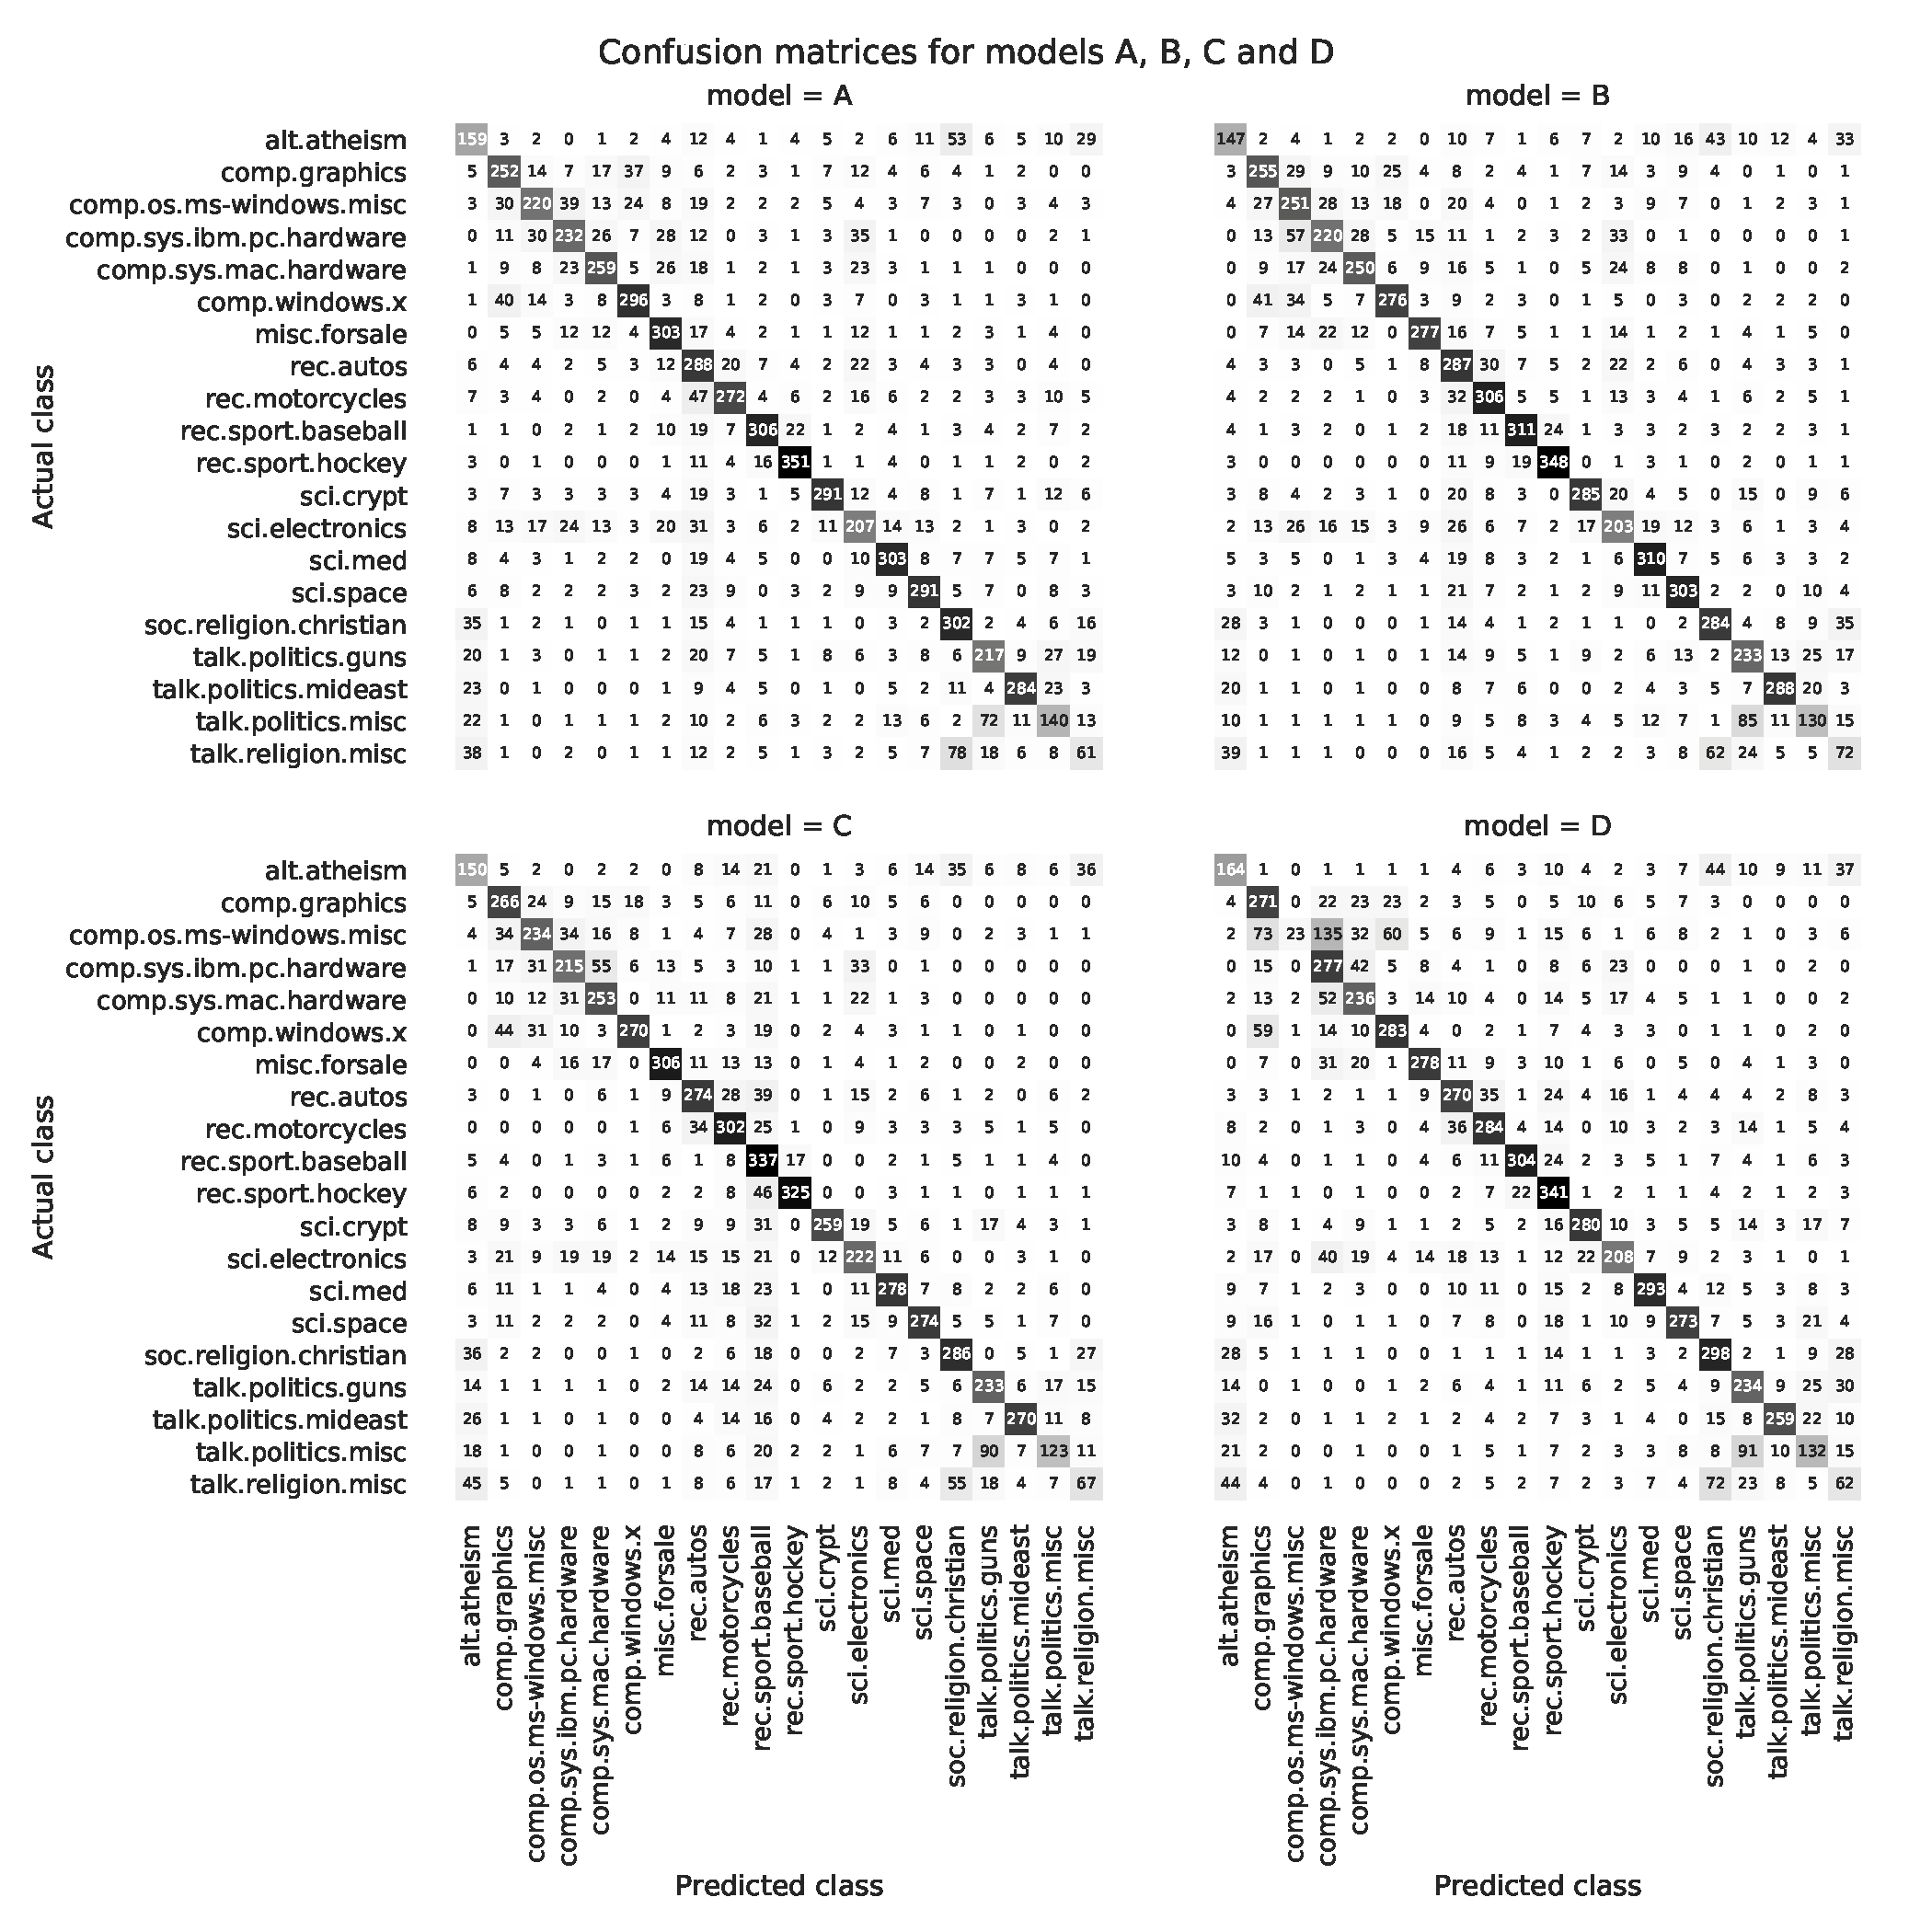
\includegraphics[width=.50\linewidth]{images/chart_21.pdf} \\
\end{tabular}
\caption{Confusion matrices for models A, B, C and D}
\label{fig:confusionmatrix}
\end{figure*}

After this process we were ready to compare our scores, \textit{accuracy} and \textit{information gain}, obtained for our models A, B, C and D. However, before going into any meaningful evaluation of results, we needed to make some refinements related to variance. Altough we got through the first iteration of the presented process without such a concern, we were aware that both the hyperparameter exploration and final model training have stochastic components, and therefore our results could significantly change (as in fact they did) if we executed the exploration and training phases different times. Randomness comes in from two different sources along this process:

\begin{itemize}
    \item The neural network training process has elements that are stochastic by nature, e.g., weight initialisation, dropout regularisation, optimisation, etc.
    \item The cross-validation process can also introduce randomness if there is shuffling involved. That is the case for our Naïve Bayes classifier, for which we used shuffled cros-validation (\verb|sklearn.model_selection.ShuffleSplit|).
\end{itemize}

Quoting \cite{Zhang}, in section 5.2 giving "specific advice to practicioners": 

\say{
    When assessing the performance of a model (or a particular configuration thereof), it is imperative to consider variance. Therefore, replications of the cross-fold validation procedure should be performed and variances and ranges should be considered.
}

\subsection{Refinement}\label{sec:refinement}
Thus, we repeated the whole process but \textbf{including variance} in the analysis. First, in the hyperparameter selection process, we repeated the training session \textbf{5 times} for each hyperparamter combination and \emph{we considered a \textbf{confidence level of 95\%} and confidence intervals of validation accuracy values to make decisions about best hyperparameter combinations}. And then, once the best hyperparameter combination was selected, we ran the final training session \textbf{10 times} for each model and again we compared the resulting values for \textit{accuracy} and \textit{information gain} taking confidence intervals into account with the same alluded confidence level. In section \ref{sec:results} we bring all this up together.

%%
%%
%%
\section{Results}\label{sec:results}
\subsection{Model Evaluation and Validation}

\begin{table}[h]
    \centering
    \resizebox{\textwidth}{!}{%
    \begin{tabular}{||c | c | c | c | c | c ||}
        \hline
        Hyperparameter & Description & Model A & Model B & Model C & Model D \\
        \hline
        \hline
        \verb|epochs & num. epochs (explore) &  20 & - & - & - \\
        \verb|epochs & num. epochs (train) & 30  & 30 & 1,000 & - \\
        \hline
        \verb|optimizer & optimizer &  nadam & nadam & nadam & - \\
        \verb|batch\_size & batch size & 128  & 128 & 128 & - \\
        \hline
        \verb|embedding\_preload & preload \textit{GloVe} embeddings & True & True & True & - \\
        \verb|embedding\_train & train embeddings layer & True & True & True & -  \\
        \hline
        \verb|cnn\_filter\_size & CNN filter size (filter region size) & 2 & 1 & - & - \\
        \verb|cnn\_num\_filters & num. convolutional filters (feature maps) & 600 & 600 & - & - \\
        \hline
        \verb|alpha & additive (Laplace/Lidstone) smoothing parameter  & - & - & - & 0.8 \\
        \hline
        
    \end{tabular}
    }
    \caption{Best hyperparameter values for models A, B, C and D}
    \label{tab:besthyperparams}
\end{table}

In table \ref{tab:besthyperparams} we summarize the best hyperparameter values for our models A, B, C and D after the hyperparameter exploration process. For getting the best hyperparamter combination for Model A we followed the process described in section \ref{sec:trainingmodelA}. The first step of the phased grid search was about finding the best optimizer and batch size. In Figure \ref{fig:explorationphase0}, left side, we visualize the validation accuracies for the considered optimizers (rmsprop, adagrad, adam, nadam) and batch sizes (64, 128, 256 and 512). The figure shows that the best combination seems to be for the \textbf{nadam} optimizer and batch size of \textbf{128}. However note that the confidence interval (95\%) of this combination overlaps with the ones for (nadam, 64) and (nadam, 256). We chose the combination (nadam, 128) as the most likely best one, but we cannot affirm that assuming our confidence level of 95\% this selection of hyperparamter values is better than the other two. In the second phase of the exploration, with optimizer and batch size fixed to (nadam, 128), we explored the embeddings layer. Figure \ref{fig:explorationphase0}, right side, shows the results for the two related hyperparamters. This time the confidence intervals (95\%) are pretty narrow and do not overlap. Thus, we were quite confident to choose preloading the \textit{GloVe} embedding vectors and also training the pre-loaded embeddings layer as the best option. 
The third phase of the hyperparamter exploration is the most interesting one as it deals with number and size of convolutional filters, which is where the ability to extract positional information is. In figure \ref{fig:explorationphase1}, left side, we note that the best mean for validation accuracy is above 0.72 and corresponds to a filter size 3 and 900 feature maps. However, its 95\% confidence interval overlaps with two other combinations of size and number of filters: (2,900) and (2,600), both of which have slightly lower validation accuracy means. We performed a 2-tailed t-test for combinations (3,900) and (2,600) to confirm our reasoning and it yielded a p-value of 0.3539, which is much greater than our significance level of 0.05. Thus, we can say that we had no solid base to decide which one of the 3 best combinations is better. \textbf{For this reason we chose filter size of 2 and 600 feature maps, as fewer number of filters of smaller size are expected to build a model that is less complex, therefore a model that is faster to train and less prone to overfitting}.
We applied a similar method when exploring the \textit{alpha} hyperparameter of Model D and chose 0.8 as its value because, although we got overlapping confidence intervals, it yielded the highest validation accuracy mean.

\begin{figure*}[h]
\begin{tabular}{c c}
    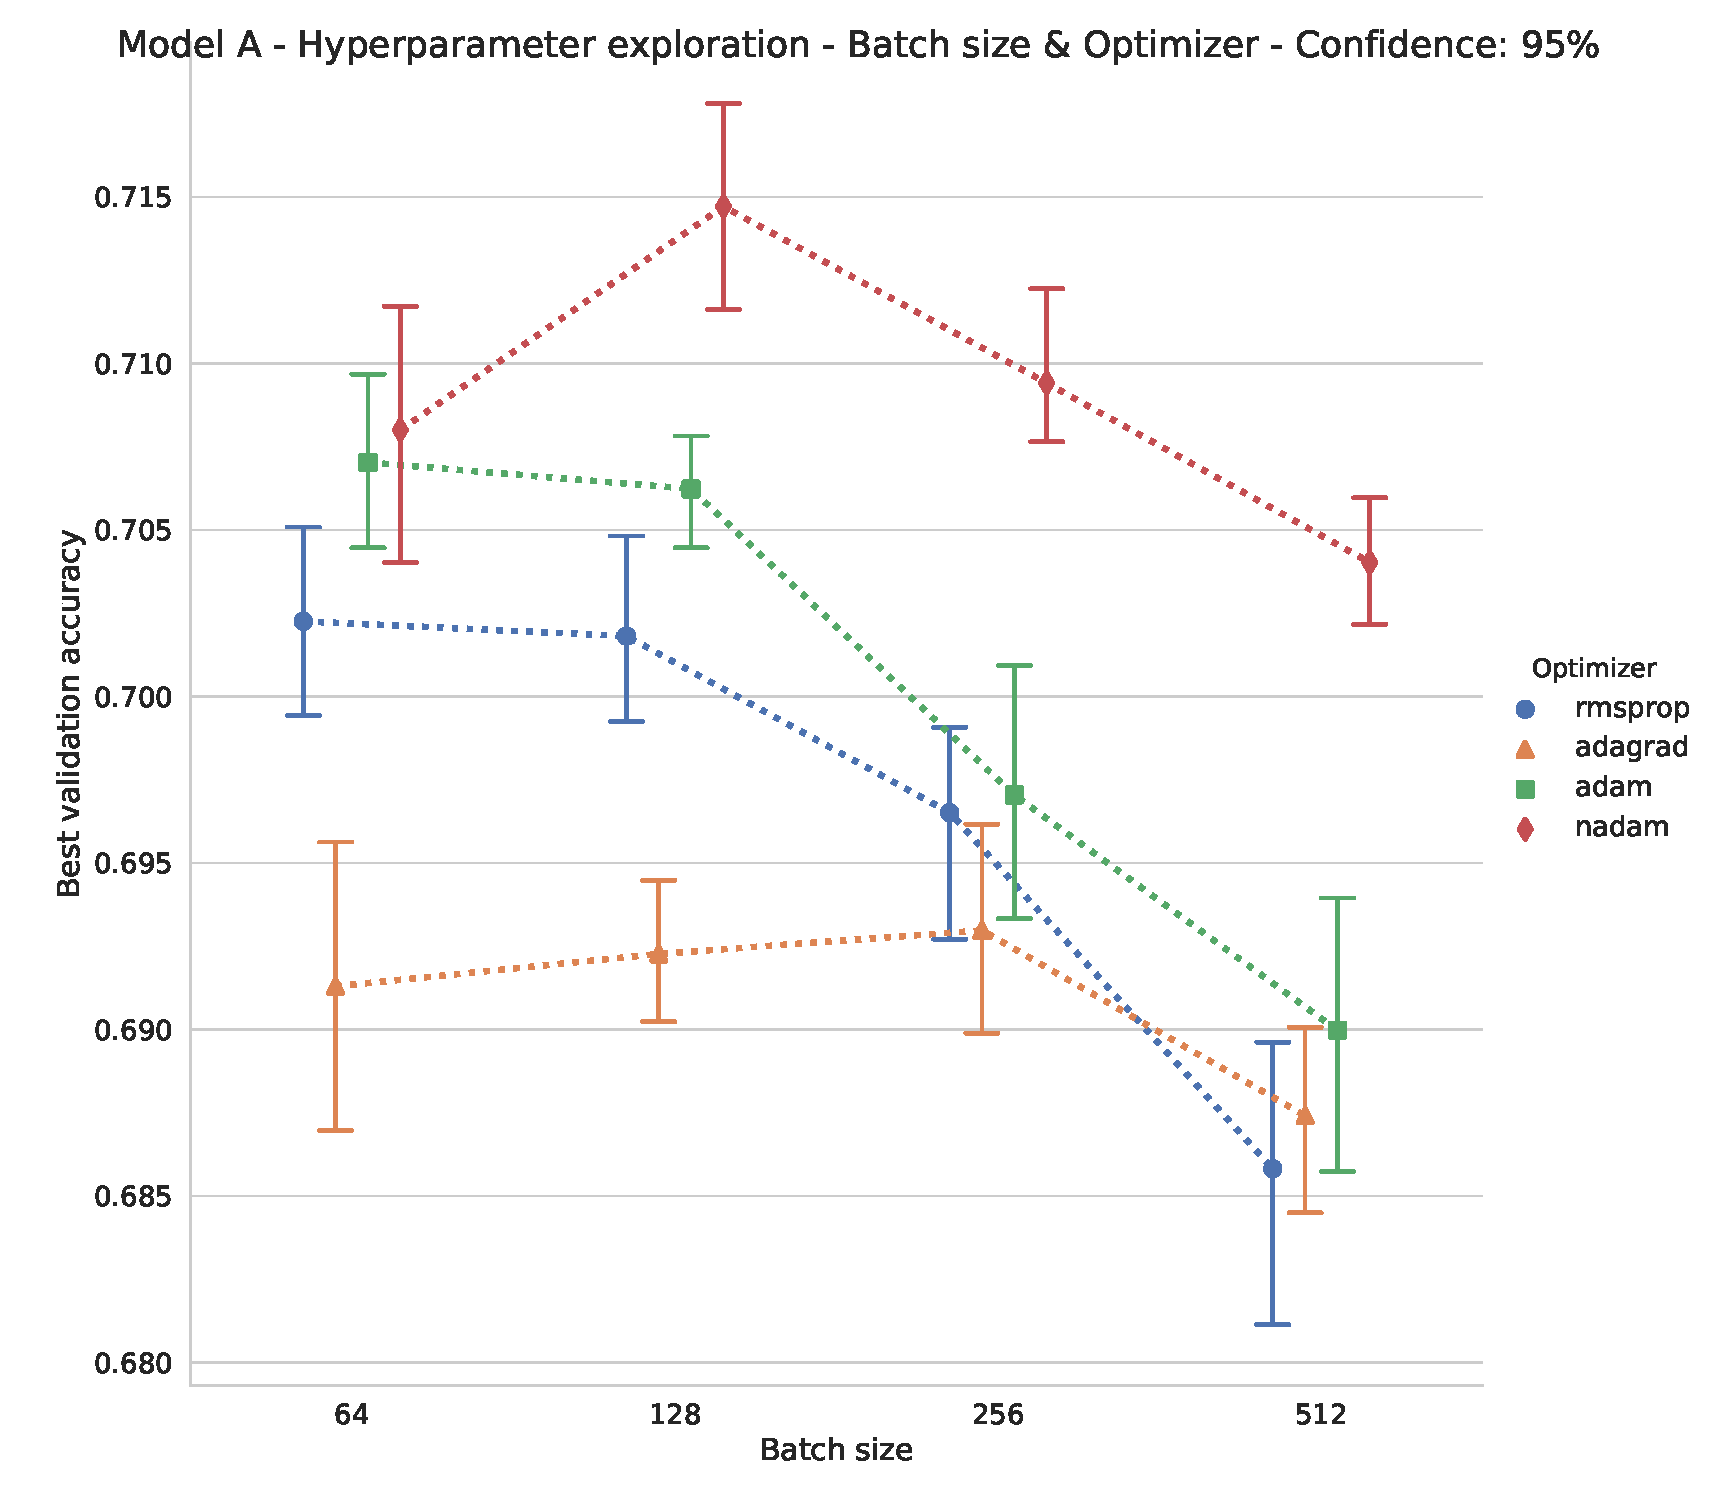
\includegraphics[width=.497\linewidth]{images/chart_09.pdf} &
    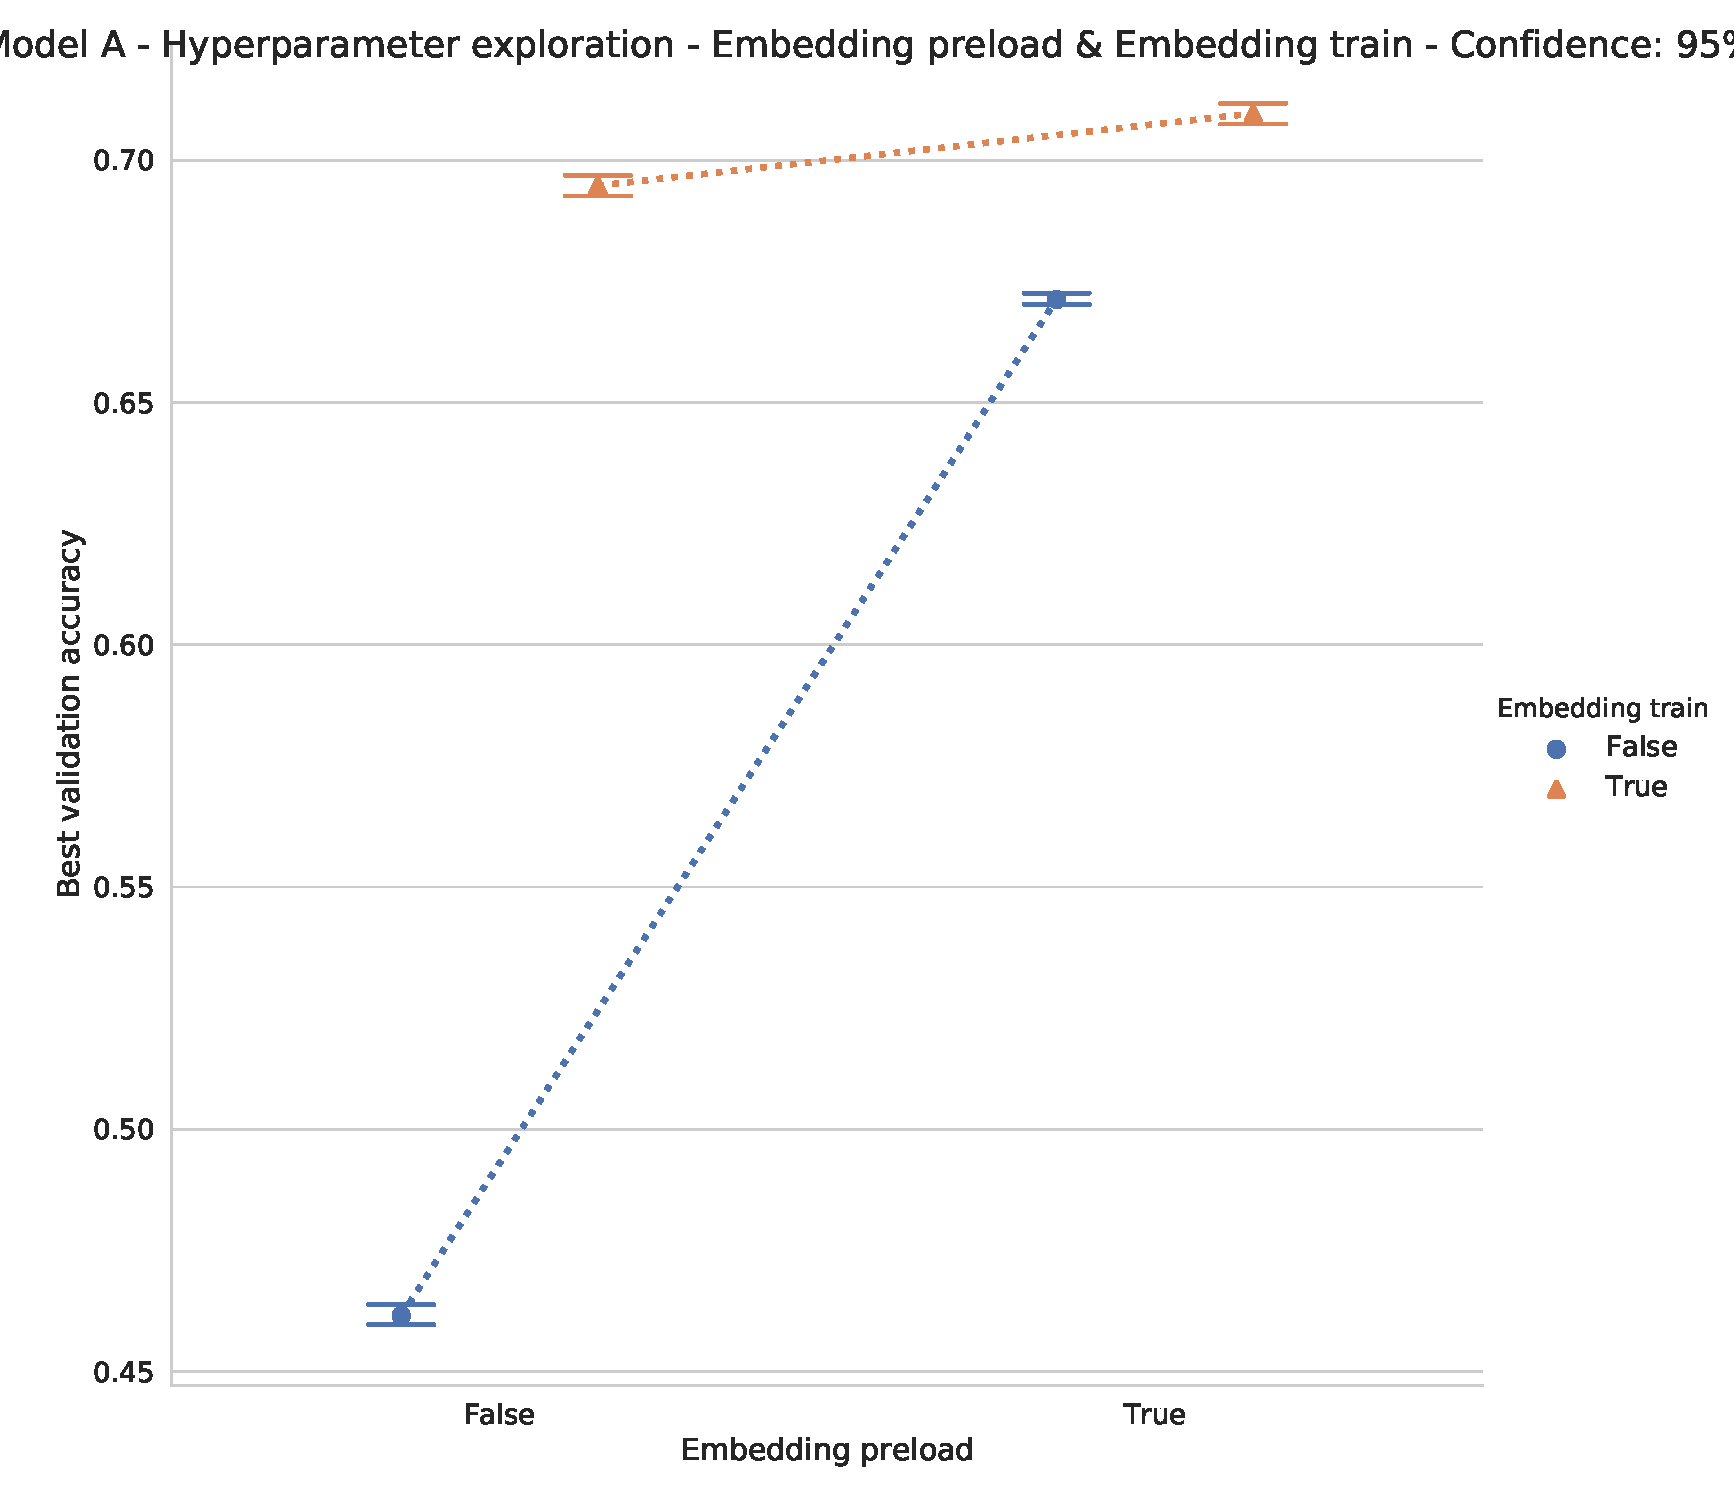
\includegraphics[width=.503\linewidth]{images/chart_12.pdf} \\
\end{tabular}
\caption{Hyperparameter exploration for Model A - Optimizer type, batch size and embeddings layer - 5 repetitions}
\label{fig:explorationphase0}
\end{figure*}

\begin{figure*}[h]
\begin{tabular}{c c}
    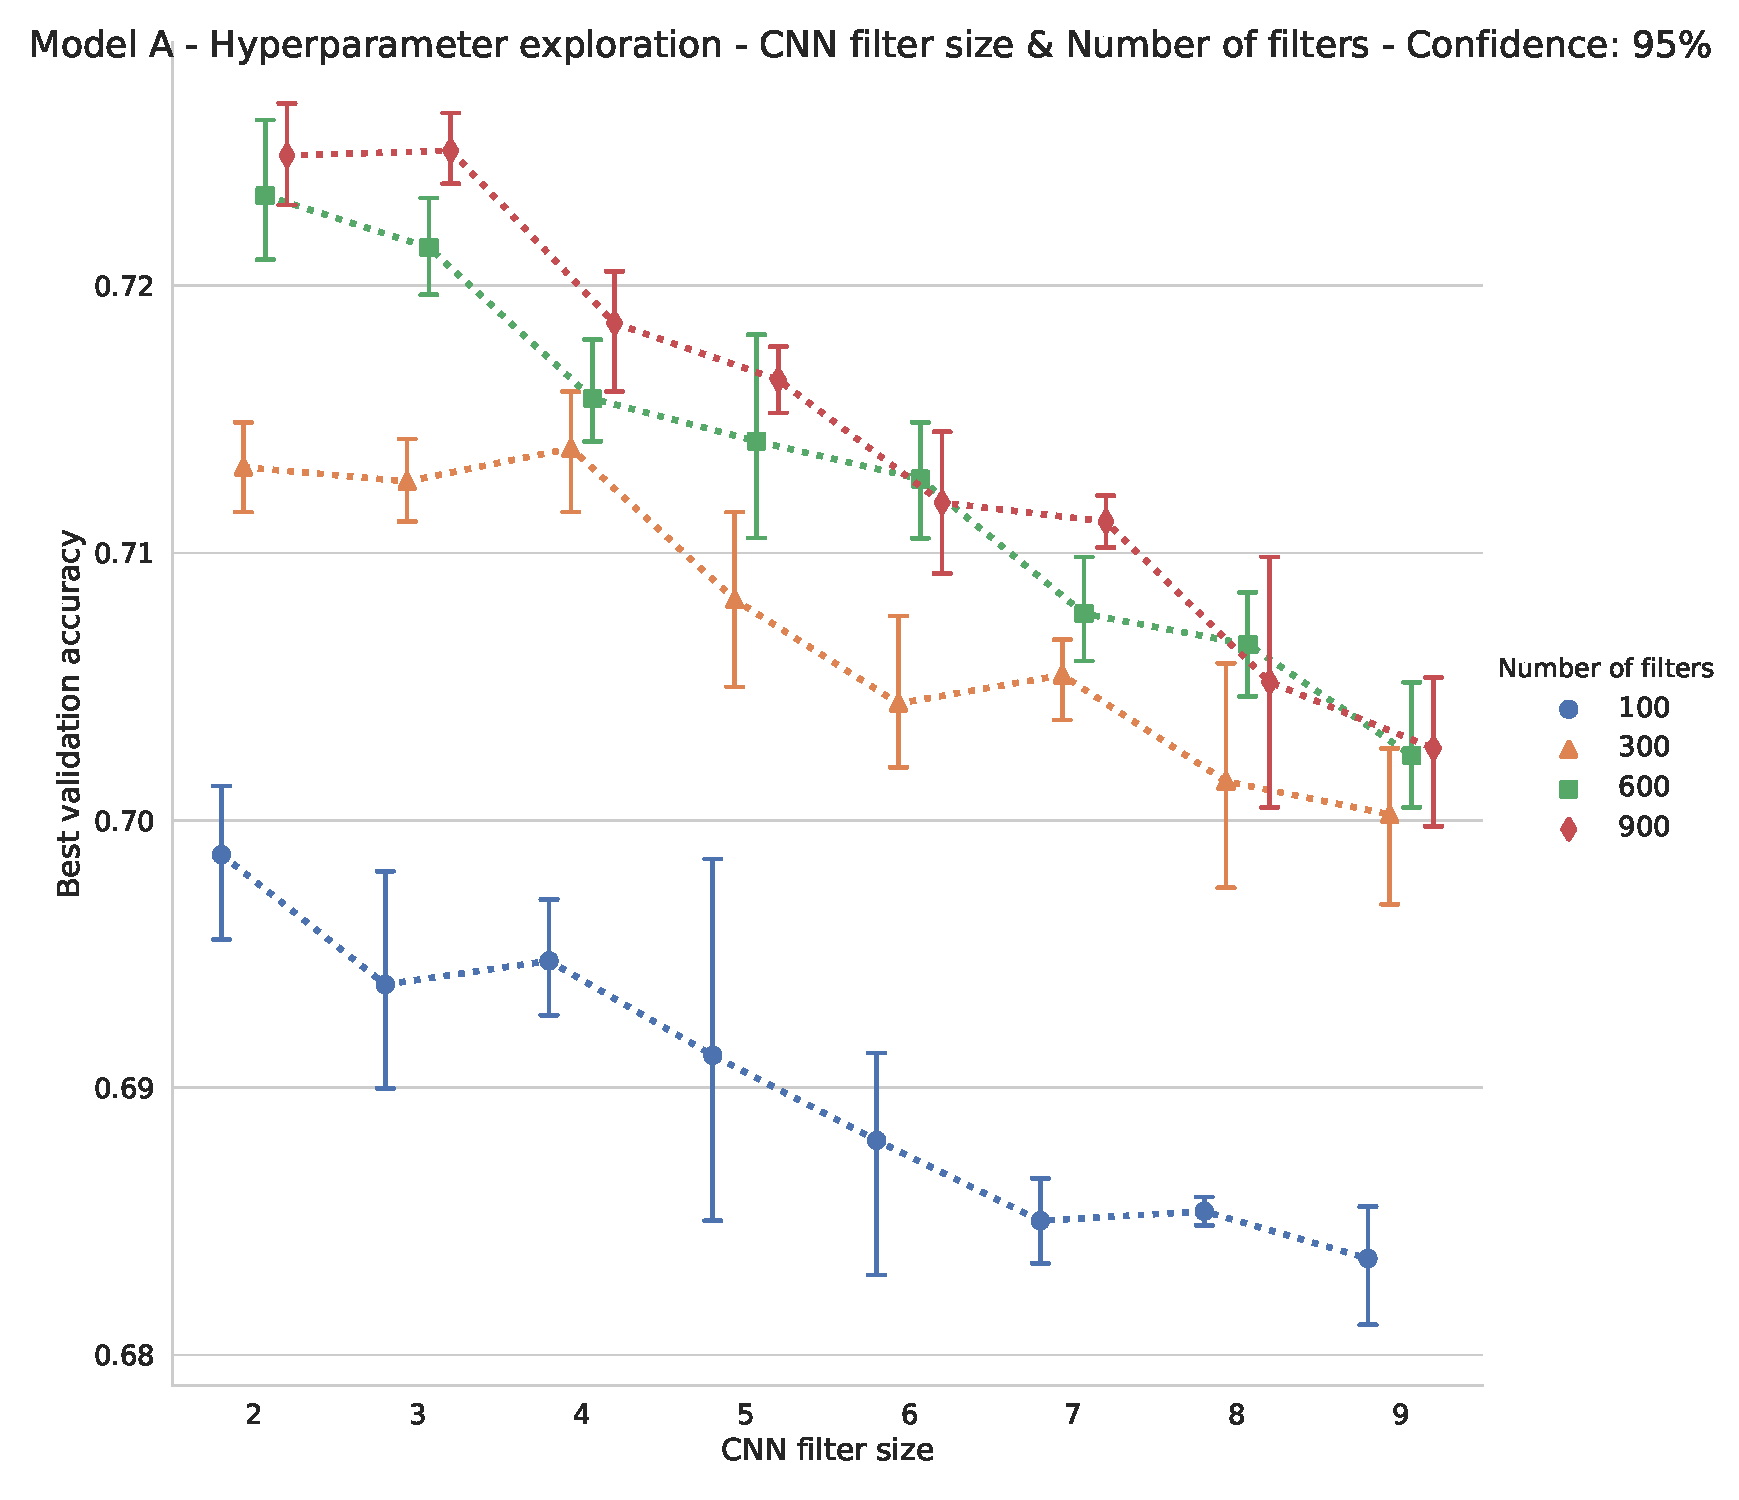
\includegraphics[width=.499\linewidth]{images/chart_14.pdf} &
    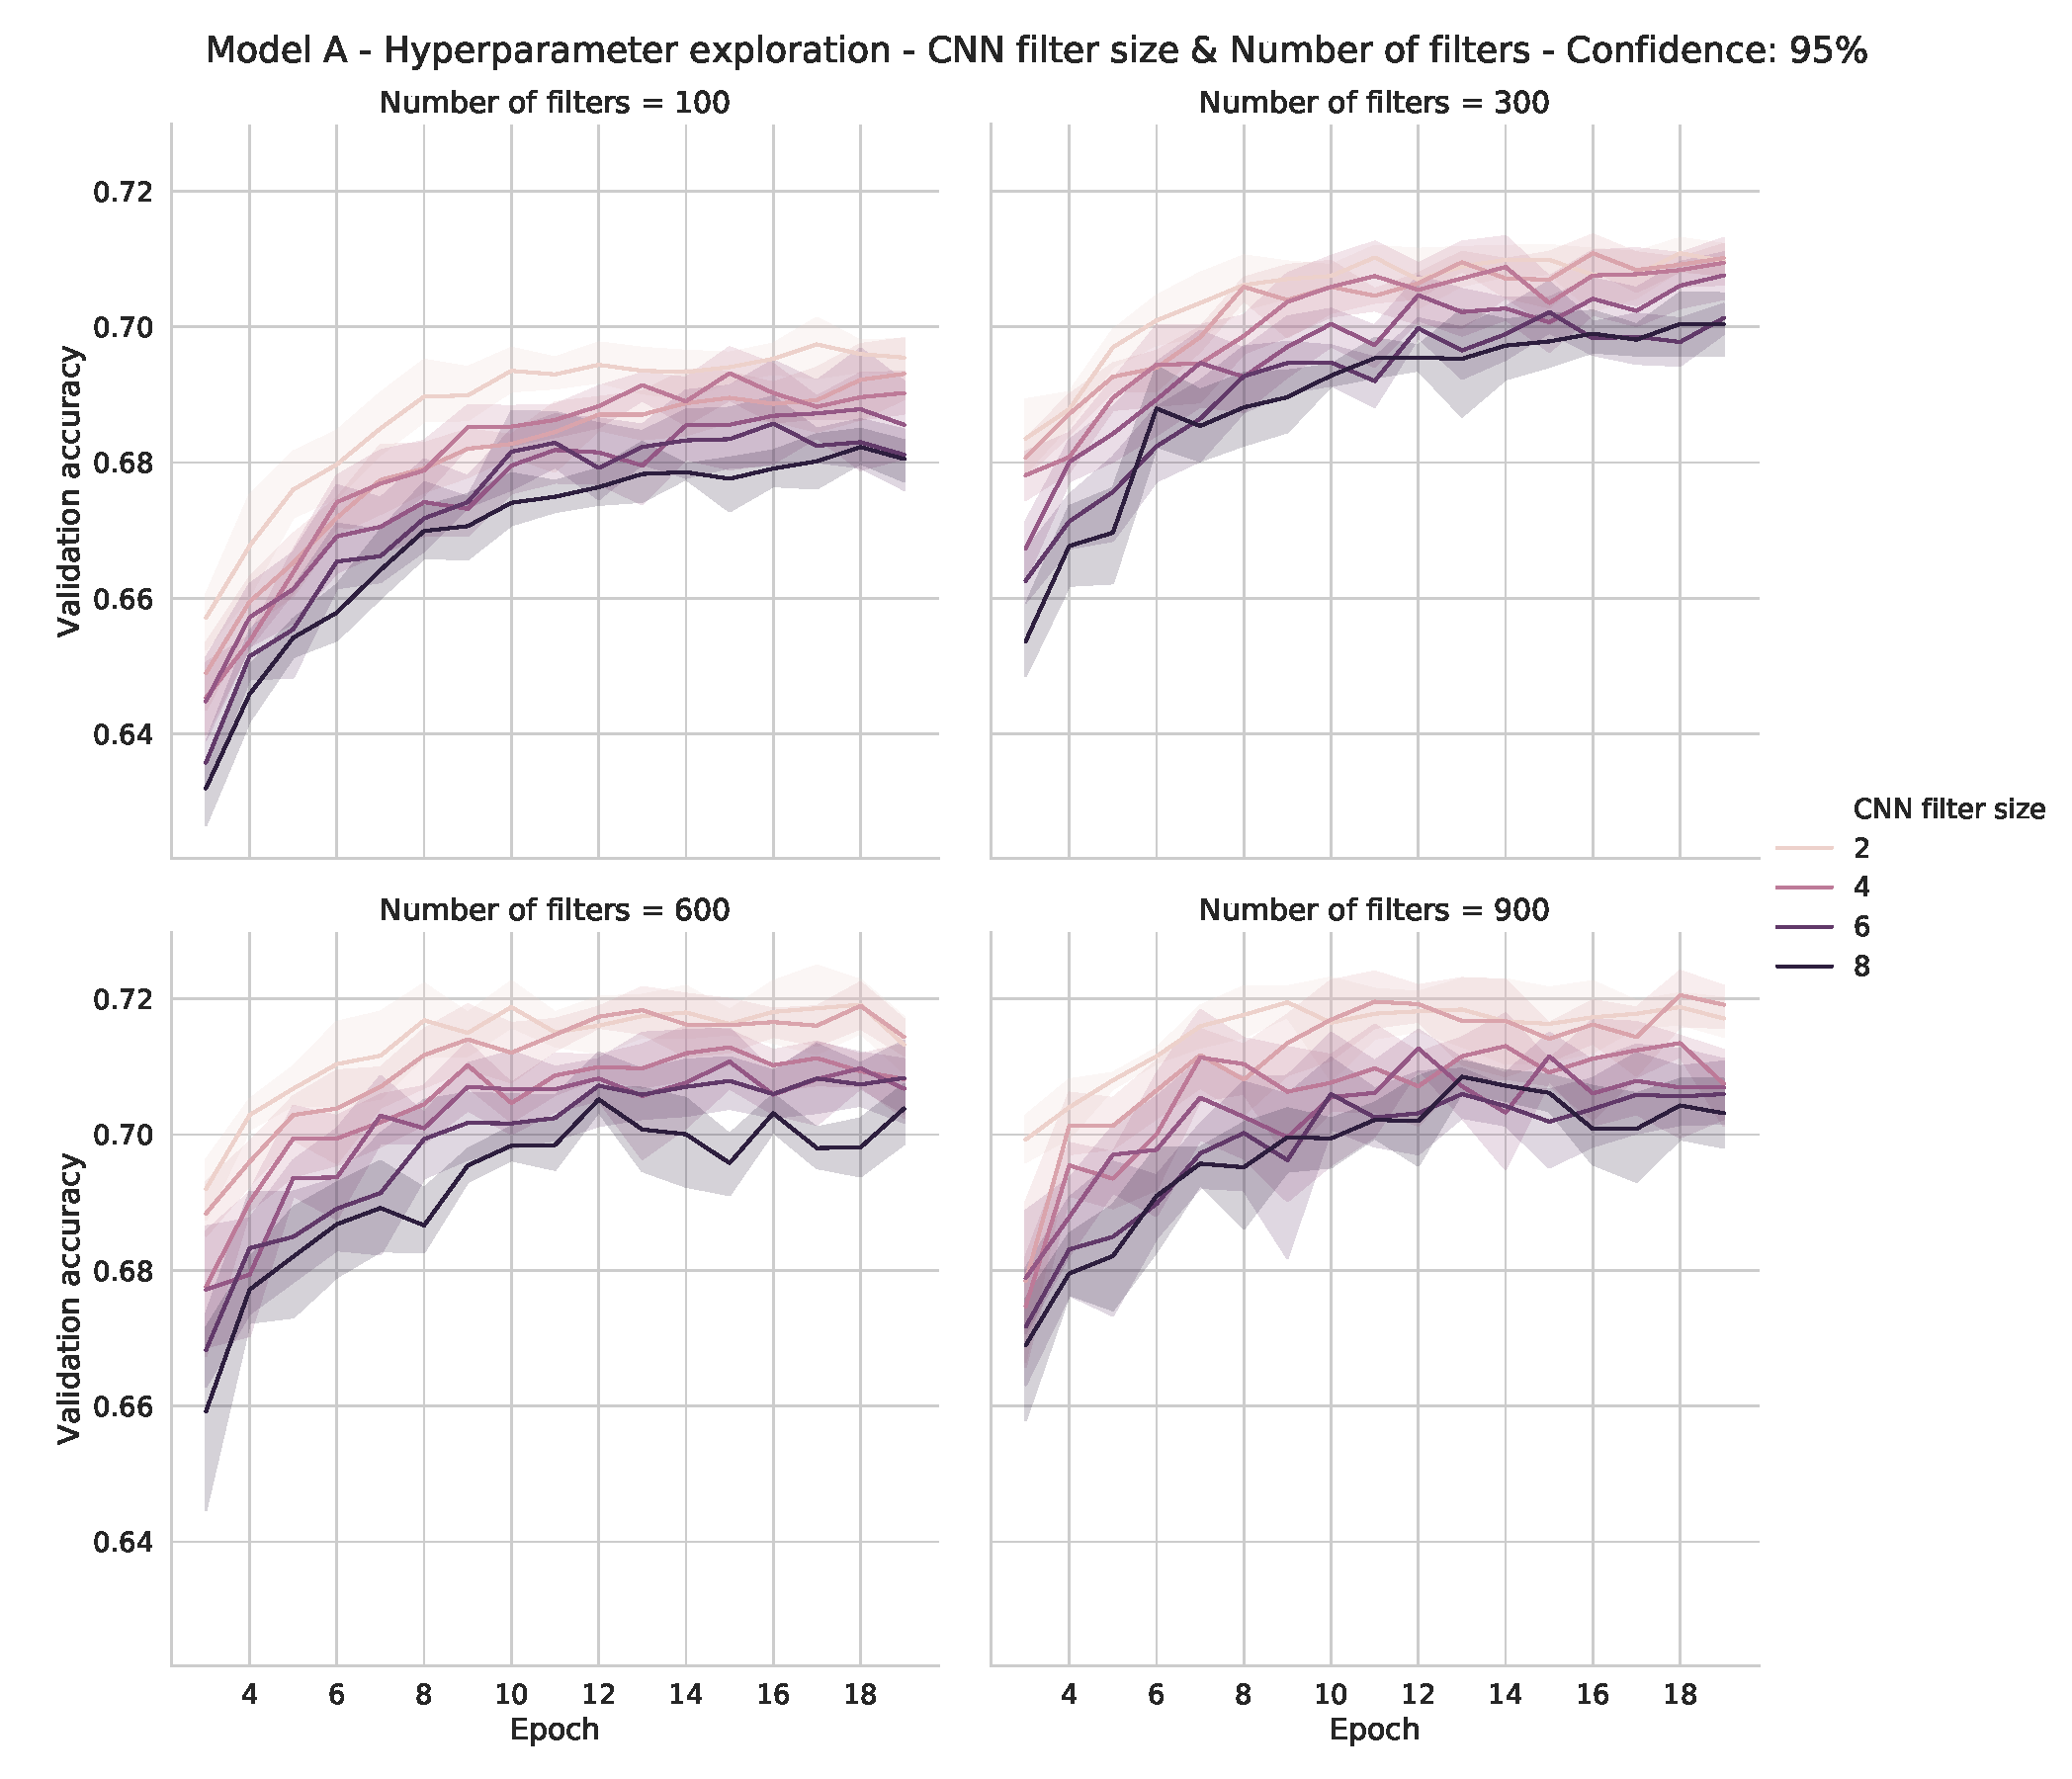
\includegraphics[width=.501\linewidth]{images/chart_15.pdf} \\
\end{tabular}
\caption{Hyperparameter exploration for Model A - Size and number of convolutional filters - 5 repetitions}
\label{fig:explorationphase1}
\end{figure*}

\subsection{Justification}\label{sec:justification}

After selecting the best hyperparameters, we went onto the process of training and evaluating each model, 10 repetitions each, to deal with variance due to stochastic processes in training and cross-validation as explained in section \ref{sec:refinement}. The results are visualized as confidence intervals in Figure \ref{fig:scores}, both for \textit{accuracy} (left) and \textit{information gain} (right). From this figure and from Table \ref{tab:results}, which lists the means for accuracy and information gain, we can make the following observations:

\begin{table}[]
    \centering
    \resizebox{.6\textwidth}{!}{%
    \begin{tabular}{||r|l||r|r||r|r||}
        \hline
         \multicolumn{2}{||l||}{Model} & \multicolumn{2}{l||}{Accuracy}  & \multicolumn{2}{l||}{Information Gain} \\
         \hline
         \hline
         A & CNN (filter size 2)  & 67.1 \% & \textbf{+ 3.8 \%} & 2.342 bits & \textbf{+ 0.105 bits} \\
         B & CNN (filter size 1) & 65.8 \% & + 2.5 \% & 2.292 bits & + 0.055 bits \\
         C & Dense NN & 66.0 \% & + 2.7 \% & 2.316 bits & + 0.079 bits \\
         D & Naïve Bayes & 63.3 \% &  & 2.237 bits &  \\
         \hline
    \end{tabular}
    }
    \caption{Mean Accuracy and Information Gain per model and improvement over Naïve Bayes classifier - 10 repetitions}
    \label{tab:results}
\end{table} 

\begin{itemize}
    \item Model A shows the best results, both for \textit{accuracy}, 67.1\%, and \textit{information gain}, \textbf{2.342 bits} (to be subtracted from the original entropy of the dataset, 4.314 bits). 
    \item Model C shows the worst score, as expected. \textit{Accuracy} of 63.3\% (3.8\% worse than Model A), and \textit{information gain}, \textbf{2.237 bits} (0.105 bits worse than Model A).
    \item Model B and C lie somewhere in the middle both in terms of \textit{accuracy} and \textit{information gain}.
    \item Within our confidence level (95\%) we are quite confident that Model A is significantly better than the rest of them, and that Model D is significantly worse. See how their confidence intervals (A and D) do not overlap with any other model.
    \item Within our confidence level, we cannot affirm that model B is better than C nor C better than B. Whereas for information gain the confidence intervals do not overlap, for accuracy they do.
    \item We formalized the observations above by performing a 2-tail t-test for all possible model combinations. Figure \ref{fig:pvalues} shows the p-values we obtained. Observe how the only case in which the p-value is higher than the significance level (0.05) is the combination of models B and C, for which the p-value is 0.11 (greater than 0.05). Therefore we cannot reject the \emph{null hypothesis} in this case and cannot say that any of the two models (B and C) is better than the other.
\end{itemize}

The main takeaway here is that we have proved that \textbf{our convolutional model with 600 convolutional filters of size 2 (Model A) is not only better than the other 3 models in terms of accuracy and information gain, but also that we have some basis to affirm that it can extract some additional information which is positionally encoded}, and which the rest of the models (B, C and D) cannot extract. However, we have to be aware according to Table \ref{tab:results} that the improvement in accuracy is around 1.3\% over model B, and \textbf{the extra information over model B is only 0.05 bits}. We see two interpretations to this:
\begin{itemize}
    \item either that our model is relatively good extracting positional information from text but there is not a lot of positional information to be extracted in our dataset \footnote{I.e., information relevant to the classification task and specific dataset.},
    \item or that there is more positional information than 0.05 bits in our dataset but our convolutional model is not able to extract it.
\end{itemize}


\begin{figure*}[h]
\begin{tabular}{c c}
    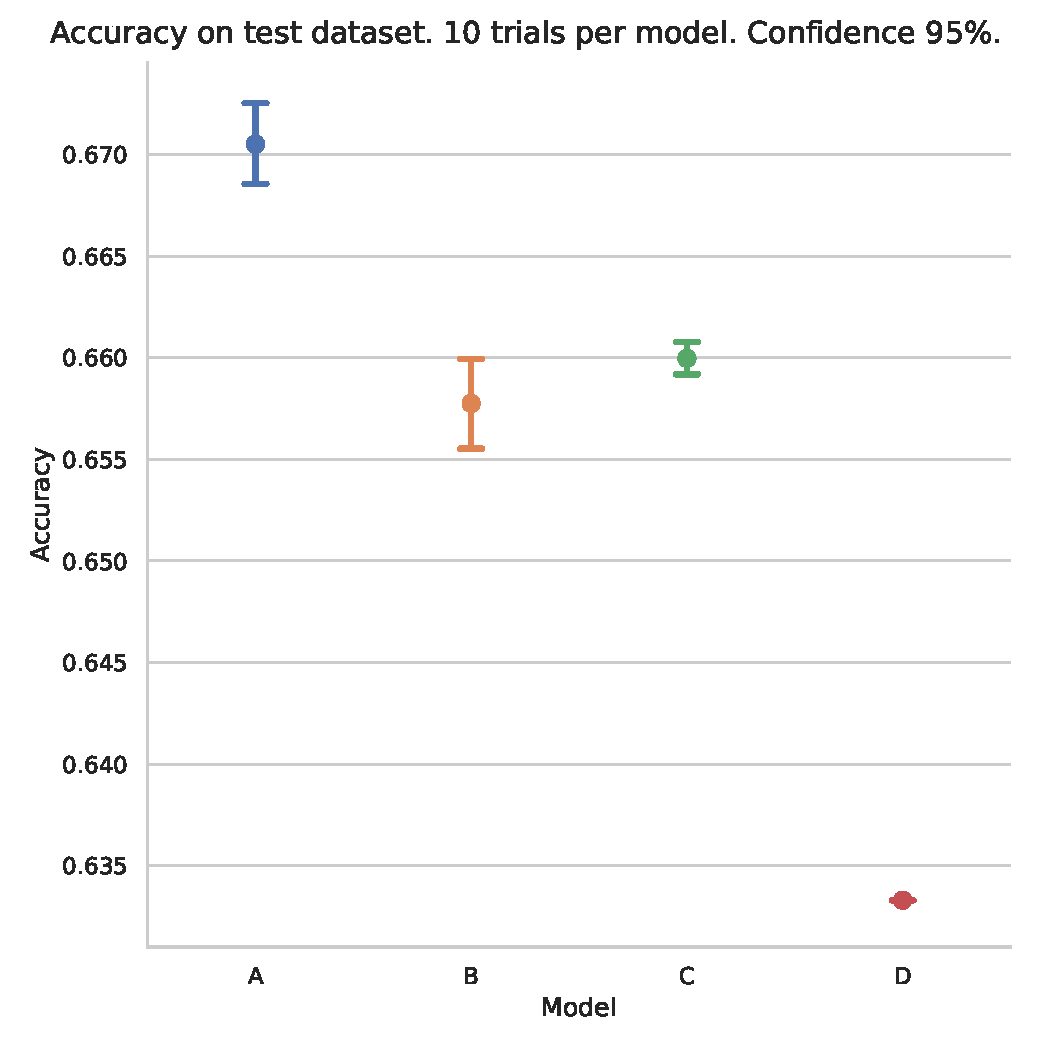
\includegraphics[width=.5\linewidth]{images/chart_26.pdf} &
    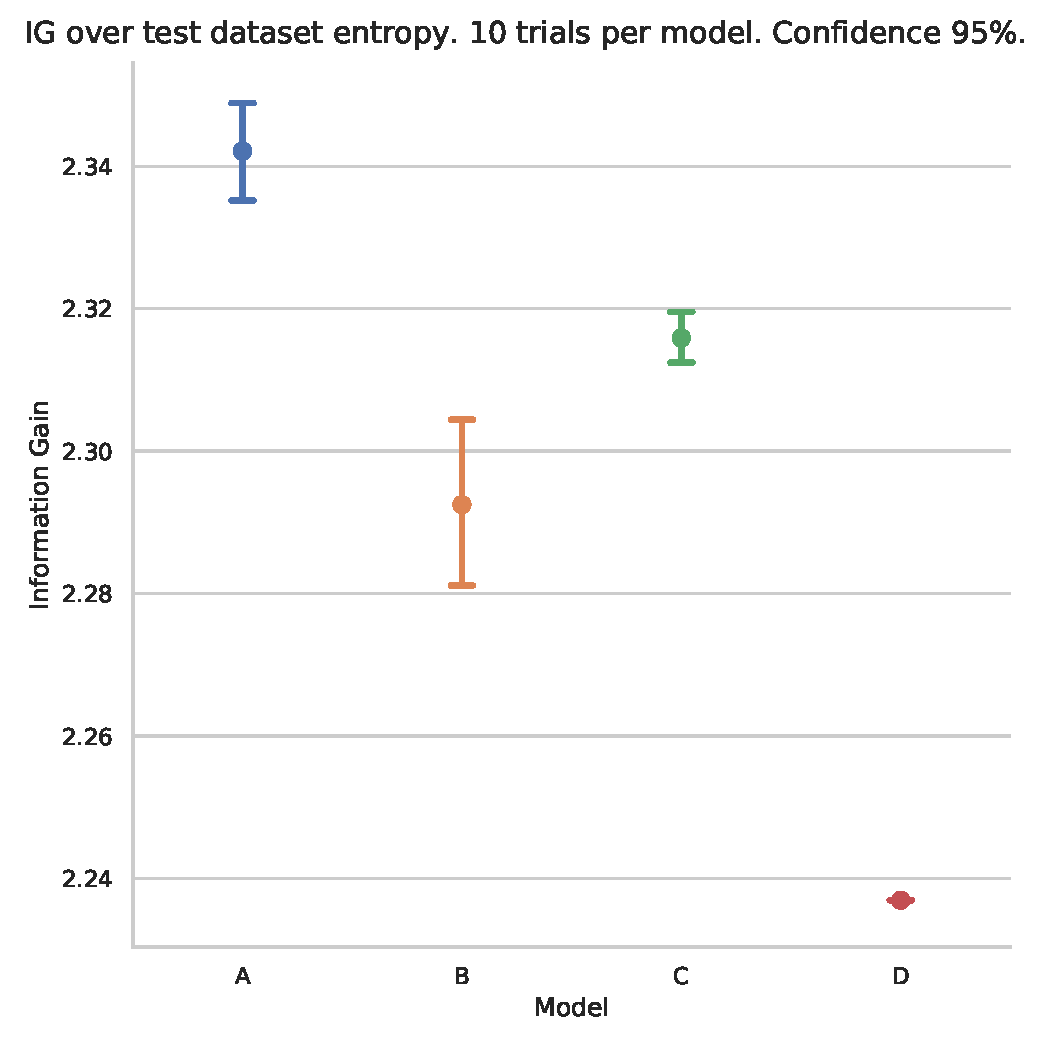
\includegraphics[width=.5\linewidth]{images/chart_25.pdf} \\
\end{tabular}
\caption{ Scores (Accuracy and Information Gain) on test dataset - 10 repetitions}
\label{fig:scores}
\end{figure*}

\begin{figure*}[h]
    \centering
    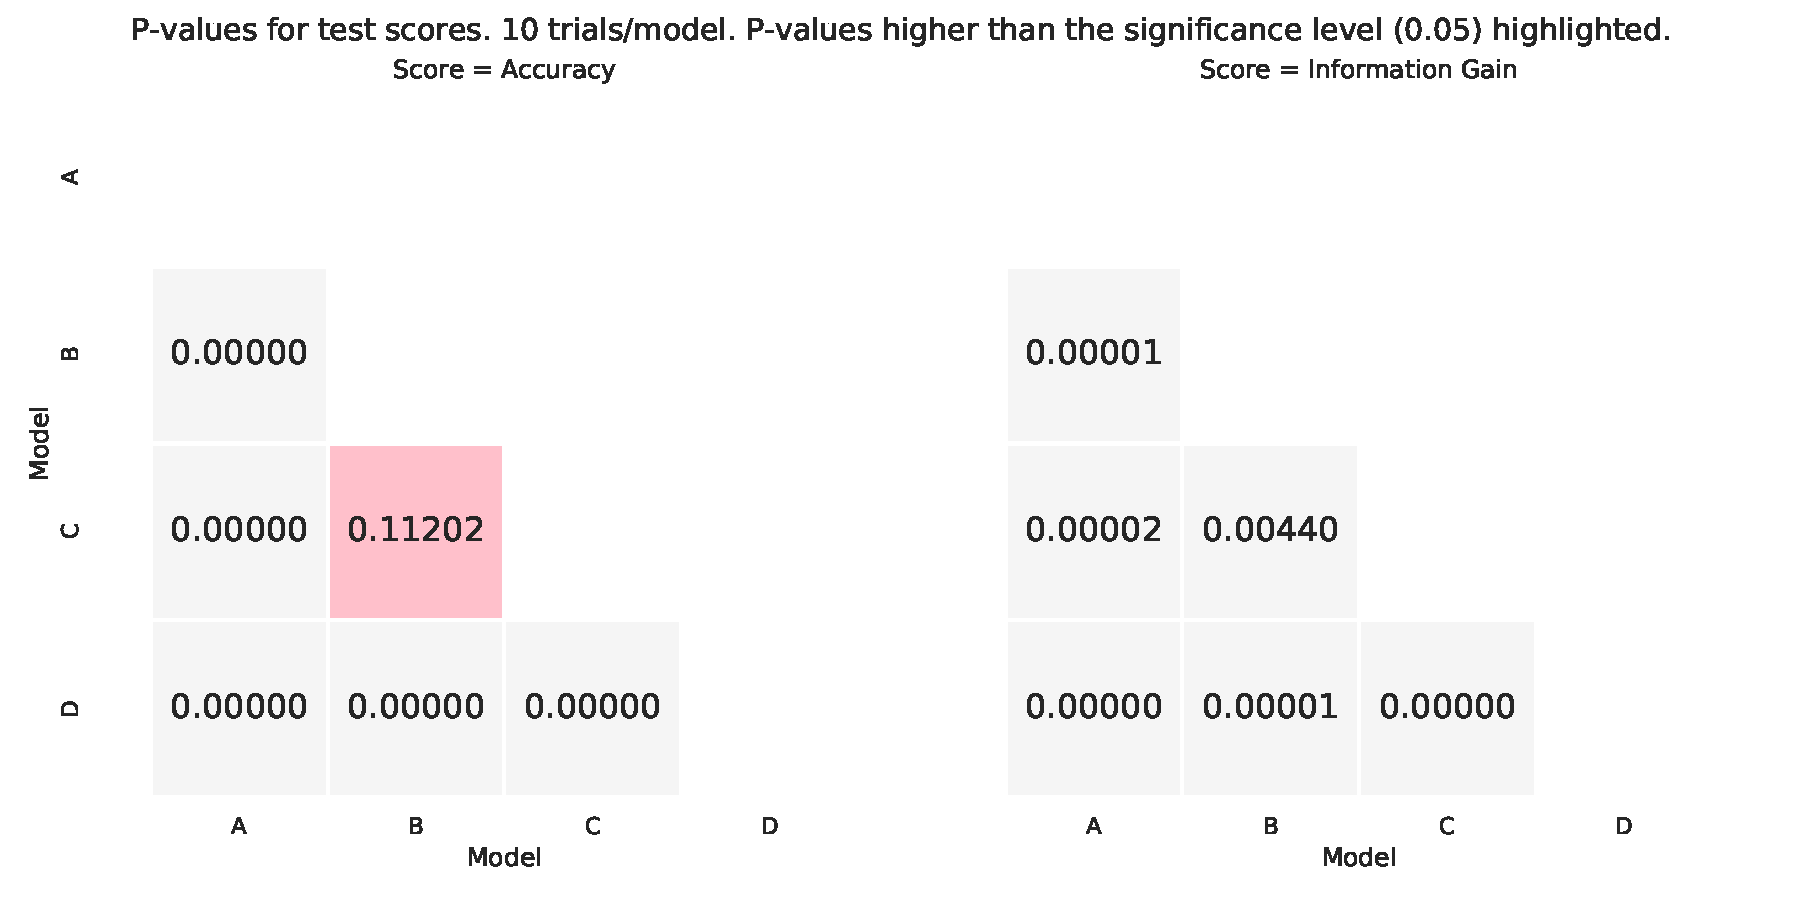
\includegraphics[width=.9\linewidth]{images/chart_28.pdf}
    \caption{P-values for Accuracy and Information Gain - 4 models - 10 repetitions each}
    \label{fig:pvalues}
\end{figure*}

\begin{figure*}[h]
    \centering
    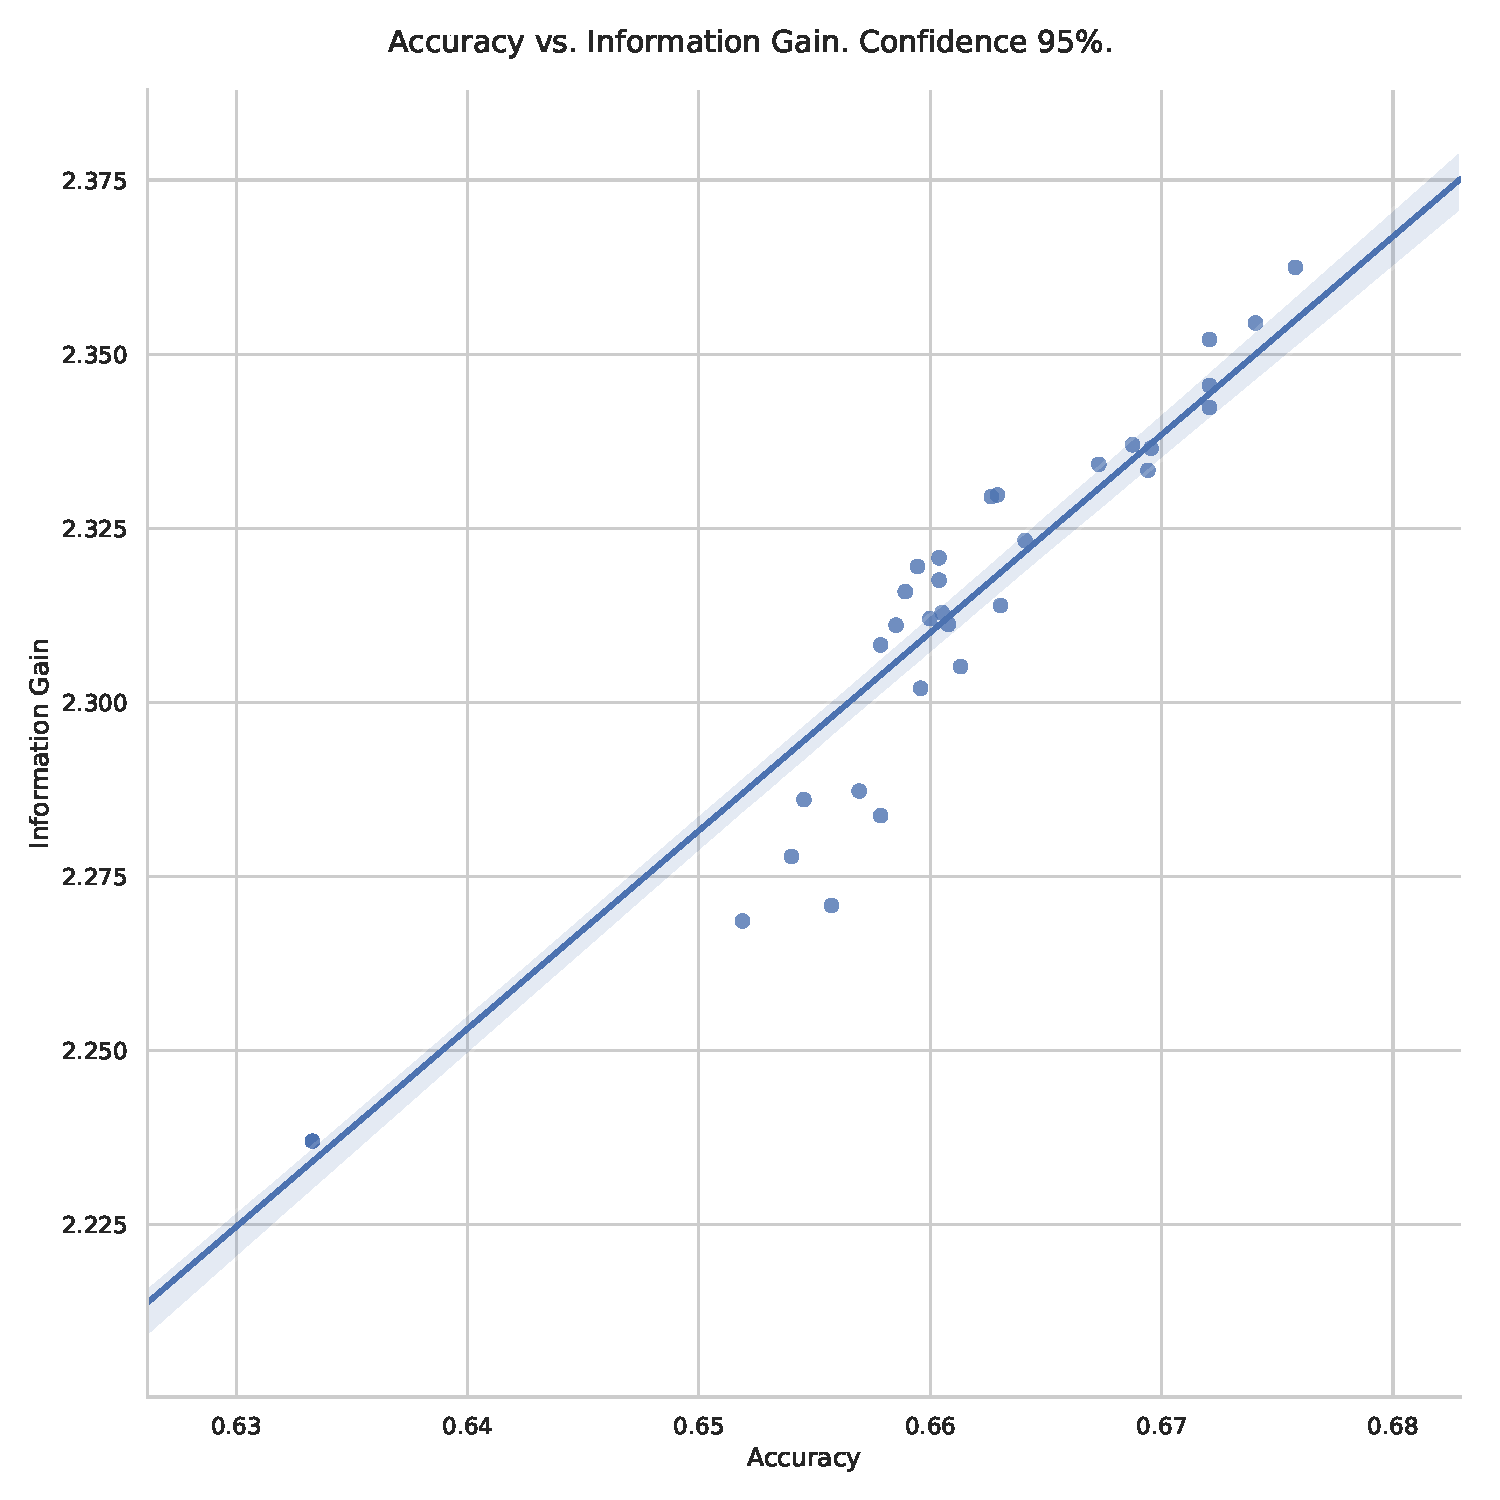
\includegraphics[width=.7\linewidth]{images/chart_27.pdf}
    \caption{Accuracy vs. Information Gain with regression - 4 models, 10 repetitions each - Pearson's r = 0.976}
    \label{fig:regression}
\end{figure*}


%%
%%
%%
\section{Conclusion}

\subsection{Reflection}

In this investigation we built a multi-class text classifier based on a convolutional neural net (CNN), tried to find an optimal configuration for it (which turned out to be 600 convolutional filters of size 2 and a trainable embeddings layer pre-loaded with \textit{GloVe} vectors of 100 dimensions), and trained it to classify documents of the \textit{20 Newsgroups dataset}. Then we compared its performance with two different carefully trimmed-down versions of itself which by design were not able to extract positional information from the documents. Our results confirmed that our CNN model can extract some positional information. However, we also realized that this improvement was modest and was mainly associated to patterns of two consecutive words (bi-grams), as models with longer filter sizes yielded worse scores. Finally, we compared our model with a standard Naïve Bayes classifier, which performed 3.8\% worse in terms of accuracy and 0.105 bits worse regarding information gain.

\begin{figure*}[h]
\begin{tabular}{c c}
    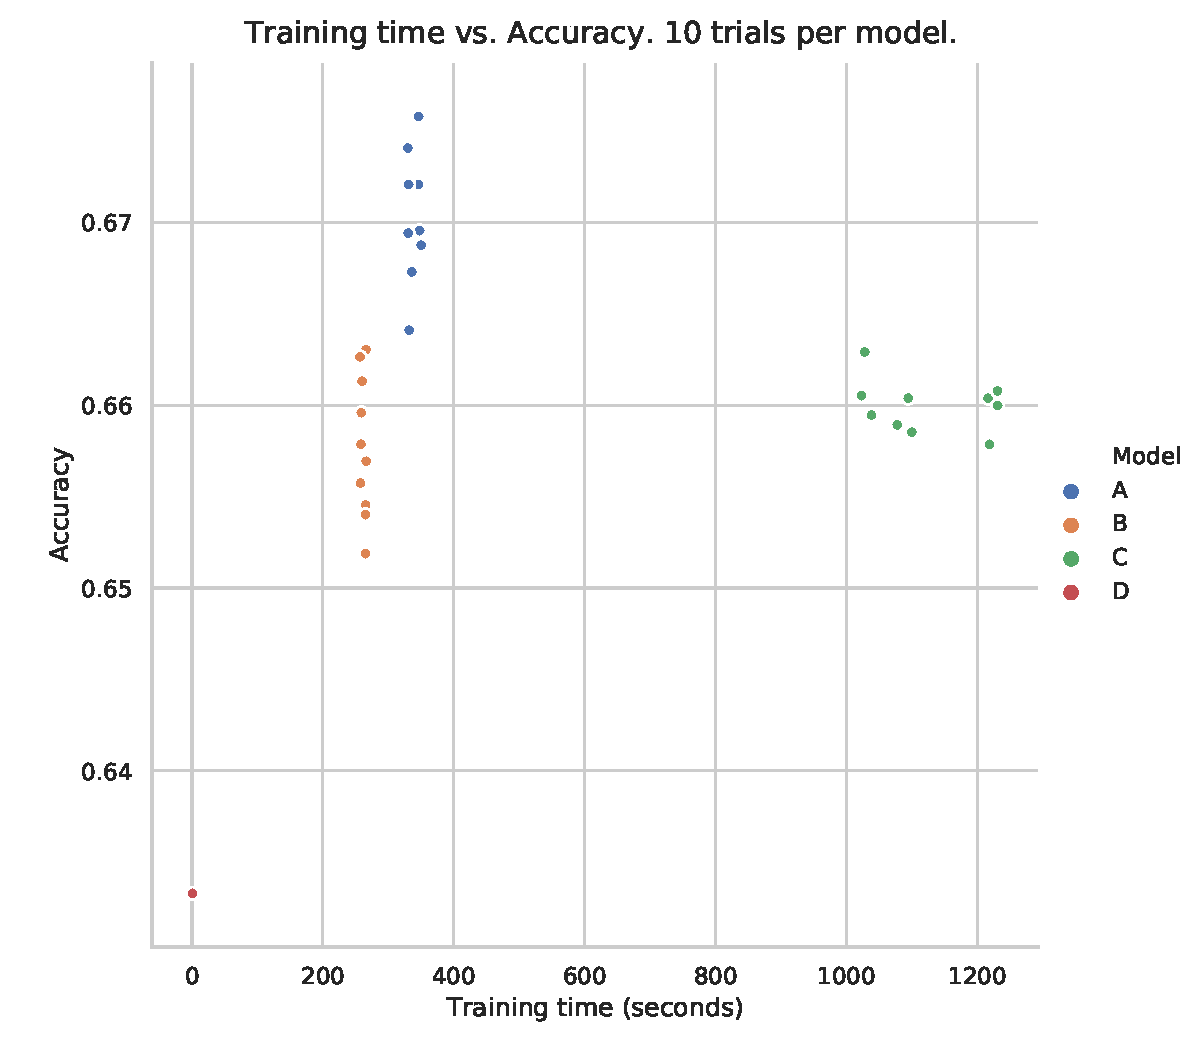
\includegraphics[width=.5\linewidth]{images/chart_29.pdf} &
    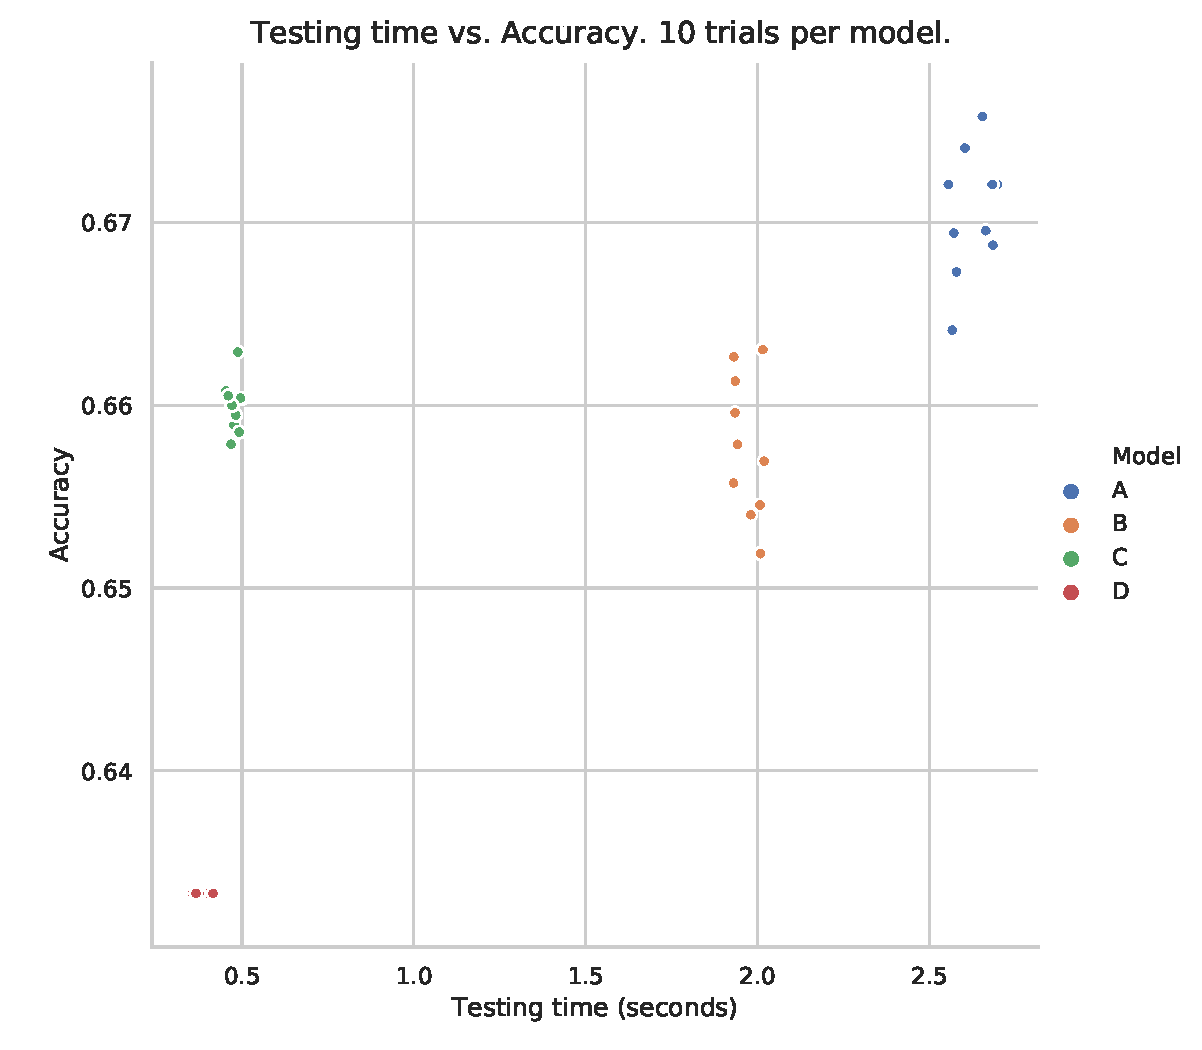
\includegraphics[width=.5\linewidth]{images/chart_30.pdf} \\
\end{tabular}
\caption{Training and testing times vs. Accuracy - 4 models -  10 repetitions}
\label{fig:times}
\end{figure*}

The question arises then, if all the extra complexity an additional resources needed by our CNN model (and even by our two trimmed-down variants) is worth it when trying to implement them in a real production environment. Along the training process, besides calculating scores (accuracy and information gain), we also gathered data about the time spent in training the model ("training time") and the time spent in calculating the accuracy score on the test dataset ("testing time") after the models were trained and loaded with the final weights. We can use these values to compare relative training and prediction speeds between models. See how Figure \ref{fig:times} visualizes both training and testing times versus the final accuracy score for each model and each repetition in the evaluation process. From these figures we can observe, without going into the detail of specific values, the following: 
\begin{itemize}
    \item The \textbf{fastest model to train and predict} is clearly Model D, the \textbf{Naïve Bayes} classifier.
    \item The \textbf{convolutional models} (A,B) are \textbf{very slow to train} ($\sim$ 300 times slower than Model D) and \textbf{slow to predict} ($\sim$ 6 times slower than model D).
    \item The \textbf{dense, non-convolutional model} (C), is \textbf{extremely slow to train }($\sim$ 1200 times slower than Model D) but \textbf{very fast to predict} (almost as fast as Model D).
    \item In addition we have to keep in mind that for these results, models A, B and C ran on GPU (Google Colab environment) and model D is built on top of Scikit-learn, which only runs on CPU. Thus, the differences between those ones and the latter must be much bigger in terms of computation resources usage.
\end{itemize}

The process of making a decision about which model is the best one ultimately depends on the concrete use case, which could justify or not the limited performance gains and the associated trade-offs in terms of time and computation resources. If we are able to assign costs and benefits to training and testing times, and also to true and false positives and negatives in our classification outcome, then we could apply the \textit{Expected Value} framework (\cite{Provost}, chapter 7) to find out which model fits better our real-world scenario in terms of profits.

Finally, we would like to enumerate some interesting aspects about this investigation that we believe are worth pointing out:
\begin{itemize}
    \item \textbf{Variance}. We learned that it is imperative to consider variance both in the hyperparamter selection process and also in performance assessment. We included confidence intervals in our analysis and visualizations, and performed t-tests and evaluated p-values in the critical parts. We also deemed it worthy to illustrate variance impact in Figure \ref{fig:explorationphase1}, right side, where we show validation accuracy trough epochs during the search for best filter size and number of filters. Observe how the validation accuracy series overlap into a blurry representation in which smaller filters seem to be better, but not clearly better, than the closest bigger ones.
    \item \textbf{Processing resources}. Training, and even evaluating neural networks, is extremely CPU intensive and, in consequence, GPU support is imperative. We had to resort to working in a Google Colab environment backed by GPUs to make it possible. Note how the variance issue aggravates the problem as it entails additional repetitions of training sessions.
    \item \textbf{Information Gain}. We proposed \textit{Information Gain} as the second evaluation score, as we believed it would best fit the problem of quantifying extraction of positional information. In figure \ref{fig:regression} we see how tightly correlated \textit{accuracy} and \textit{information gain} seem to be. We also calculated the Pearson's r value: 0.976. We would be inclined to state that in the context of our problem both scores seem to be good proxies for each other. However, in figures \ref{fig:pvalues} and \ref{fig:scores} we see that while \textit{information gain} could discriminate between models B and C with statistical significance, \textit{accuracy} could not. We find this is an interesting finding to be further researched.
    \item \textbf{Overfitting}. The best convolutional model in terms of performance turned out to be the one with the shortest filter size, 2. We learned that slightly longer filter sizes were not significantly  better and that even longer filter sizes yielded worse scores (figure \ref{fig:explorationphase1}). This can be explained if we assume that most of the positional information is encoded in bi-grams and also understanding that longer filters, even though they have the ability to \textit{emulate} shorter ones \footnote{by detecting patterns that are shorter than their length}, may easily tend to overfit and learn longer patterns from the documents that do not generalize.
\end{itemize}


\subsection{Improvement}

Finally, in order to improve and continue this work, we recommend the following lines:

\begin{itemize}
    \item Considering other models, arguably more suited to extract positional information from text, like Recurrent Neural Networks (RNN) with its variants GRU and LSTM \cite{Chollet}.
    \item Experimenting with more convolutional layers trying to give the model more abstraction power and check if that reverts into better ability to extract positional information.
    \item Validating the proposed methodology on other datasets.
    \item Considering some sort of sensitivity and robustness analysis beyond our variance analysis.
    \item And most interestingly, trying to visualize and analyze the weights of the convolutional filters obtained for our Model A, and explain them in terms of the original vocabulary of our dataset. This way we may better understand the mechanisms underlying positional information extraction and we could also get valuable insights to try to validate our hypothesis that the improvement between Model A and B has to be mainly due  to positional information.
\end{itemize}

\clearpage
\tableofcontents
\listoffigures
\listoftables
\clearpage
%\bibliographystyle{ieeetr}
%\bibliographystyle{hieeetr}
%\bibliographystyle{hapalike}
%\bibliographystyle{halpha}
\printbibliography
\nocite{*}

\end{document}